\documentclass[12pt]{article}
%\usepackage[utf8]{inputenc}
%\documentclass[UTF8]{ctexart}
%\usepackage[UTF8, heading = false, scheme = plain]{ctex}
\usepackage{geometry}
%geometry{a4paper,scale=0.9}
\geometry{a4paper,left=1cm,right=1cm,top=1cm,bottom=2cm}
\usepackage{amsfonts}
\usepackage{color}
\usepackage{url}
%\usepackage{biblatex}
\usepackage{amsmath}
\usepackage{amssymb}
\usepackage{latexsym}
\usepackage[linesnumbered,ruled,lined]{algorithm2e}
\usepackage{cite}
%\addbibresource{ref.bib}
%\bibliography{ref.bib}
\usepackage{caption}
\usepackage{graphicx, subfig}
\usepackage{float}
%\usepackage[fontset=ubuntu]{ctex}
%\usepackage{fontspec}
\usepackage{xeCJK}
%\usepackage[colorlinks,
%anchorcolor=black,
%citecolor=black]{hyperref}
%\setmainfont{SimSun}
\usepackage[section]{placeins}
\usepackage{enumitem}
\usepackage{framed}
\usepackage[framemethod=TikZ]{mdframed}
\usepackage{indentfirst}
\usepackage{setspace}%使用间距宏包
\linespread{1.5}

\title{强化学习-脉络\cite{RL_Learning_Route}}
\author{leolinuxer}
%\date{June 2020}

\begin{document}
%\setlength{\parindent}{0pt}
\maketitle
\tableofcontents

\part{强化学习的学习路线图}
\begin{figure}[H]
    \centering
    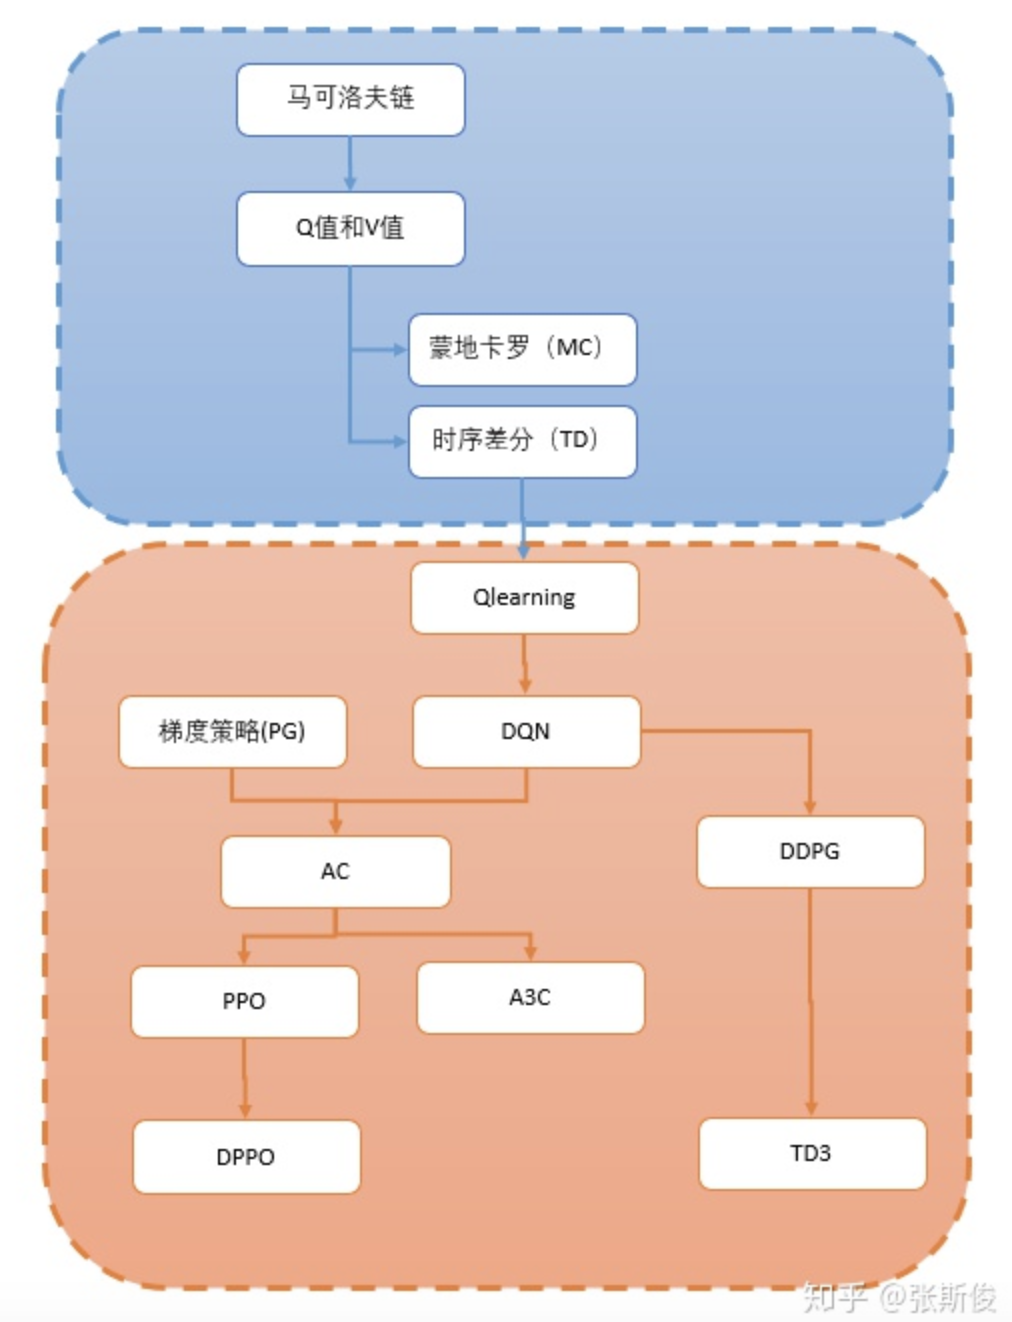
\includegraphics[width=.5\textwidth]{fig/ReinforcementLearning/RL_Learning_Route.png}
\end{figure}

\part{基础概念}
\section{马可洛夫链\cite{How_To_Understand_Markov_Chain}}
我们先来看马可洛夫链。马可洛夫链长这样子:
\begin{figure}[H]
    \centering
    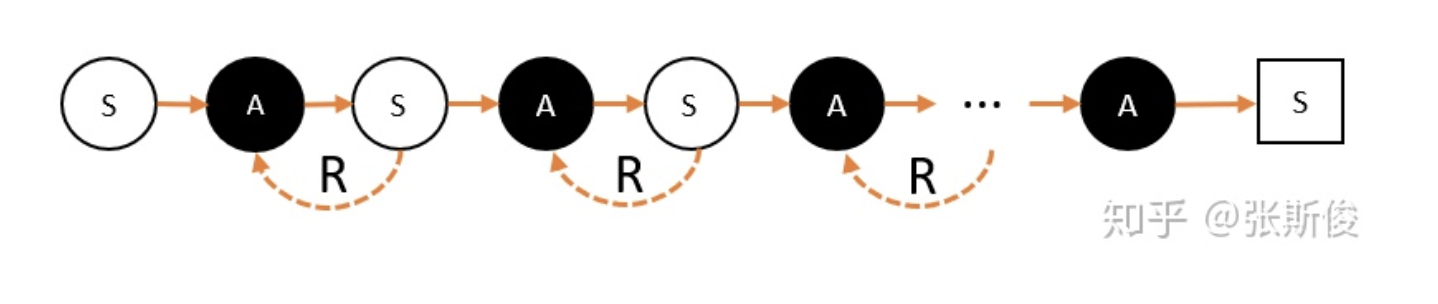
\includegraphics[width=.6\textwidth]{fig/ReinforcementLearning/RL_Markov_Chain_Example.png}
\end{figure}

\textbf{马可洛夫链描述的是智能体和环境进行互动的过程。简单说:智能体在一个状态(用S代表)下,选择了某个动作(用S代表),进入了另外一个状态,并获得奖励(用R代表)的过程}。

在马尔科夫链中,有三个重要的元素:S,A,R。我们分别来看一下,他们代表的是什么。然后大家就会明白,为什么马尔科夫链是一个很好很常用的模型。

\begin{itemize}
\setlength{\itemsep}{0pt}
\setlength{\parsep}{0pt}
\setlength{\parskip}{0pt}
    \item \textbf{S(state)状态,在图中用白色圈圈表示}。状态就是智能体观察到的当前环境的部分或者全部特征。状态空间就是智能体能够观察到的特征数量。需要特别注意的是:环境的特征可能有许多,但只有智能体能够观察到的特征才算是状态。
    \item \textbf{A(action)动作(用黑色圈圈表示)}。动作其实不用解释,就是智能体做出的具体行为。动作空间就是该智能体能够做出的动作数量。
    \item \textbf{R(reward)奖励}。当我们在某个状态下,完成动作。环境就会给我们反馈,告诉我们这个动作的效果如何。这种效果的数值表达,就是奖励。其实这里的reward翻译为“反馈”可能更合适一点。因为反馈并不是完全正面的,也有负面。
\end{itemize}

现在我们来总结一下马尔科夫链,其中也包含了强化学习的一般步骤:
\begin{enumerate}
\setlength{\itemsep}{0pt}
\setlength{\parsep}{0pt}
\setlength{\parskip}{0pt}
    \item 智能体在环境中,观察到状态(S);
    \item 状态(S)被输入到智能体,智能体经过计算,选择动作(A);
    \item 动作(A)使智能体进入另外一个状态(S),并返回奖励(R)给智能体。
    \item 智能体根据返回,调整自己的策略。 重复以上步骤,一步一步创造马尔科夫链。
\end{enumerate}

所以,我们希望通过让智能体在环境里获取最多的奖励,把智能体训练成我们想要的样子——就是能完成某些特定的任务。

所以,我们马上遇到第一个坑:马尔科夫链,其实应该叫马尔科夫树吧!
\begin{figure}[H]
    \centering
    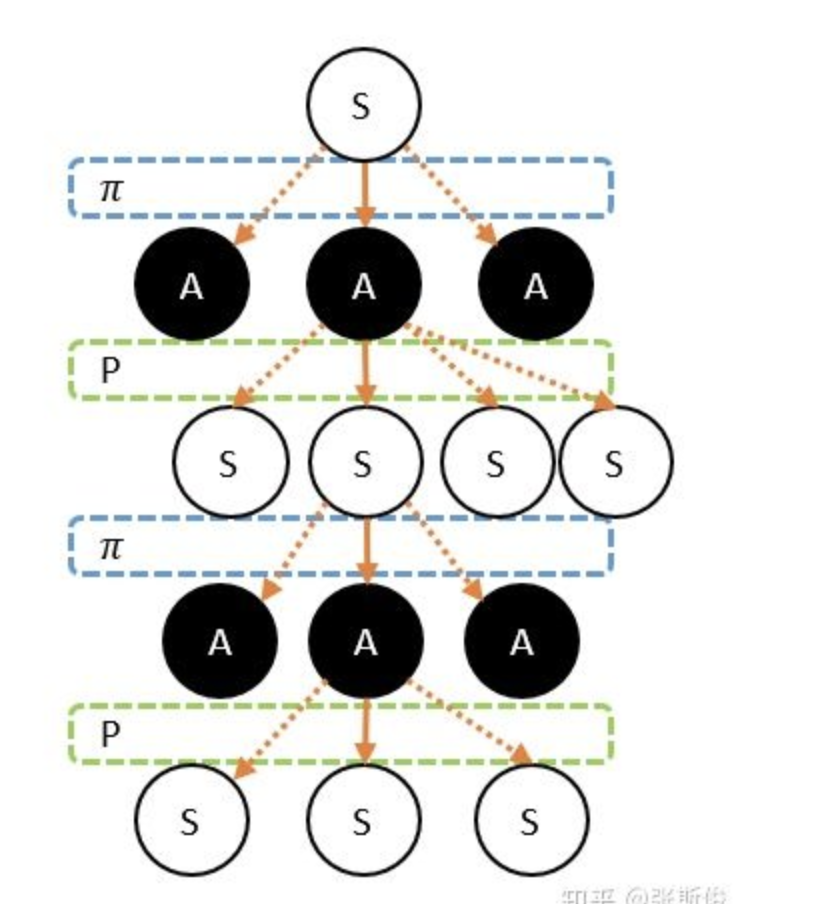
\includegraphics[width=.5\textwidth]{fig/ReinforcementLearning/RL_Markov_Chain_Tree-Example.png}
\end{figure}

其中,$\pi$代表选择策略的概率分布;$P$代表状态转移的概率分布;

我们看到的链,是因为我们从现在往后看,但如果往前看,是充满不确定性的。这里的不确定性包括两方面:

(1). 智能体的行动选择(策略):智能体的每次选择都不是固定的,而是按照一定的策略分布。这个概率分布我们称为策略,用$\pi$表示。

(2). 状态转移概率(环境的不确定性):这个只跟环境有关关系。例如飞行棋的掷骰子游戏,我们执行同样的动作,也有可能进入不同的状态。

\begin{figure}[H]
    \centering
    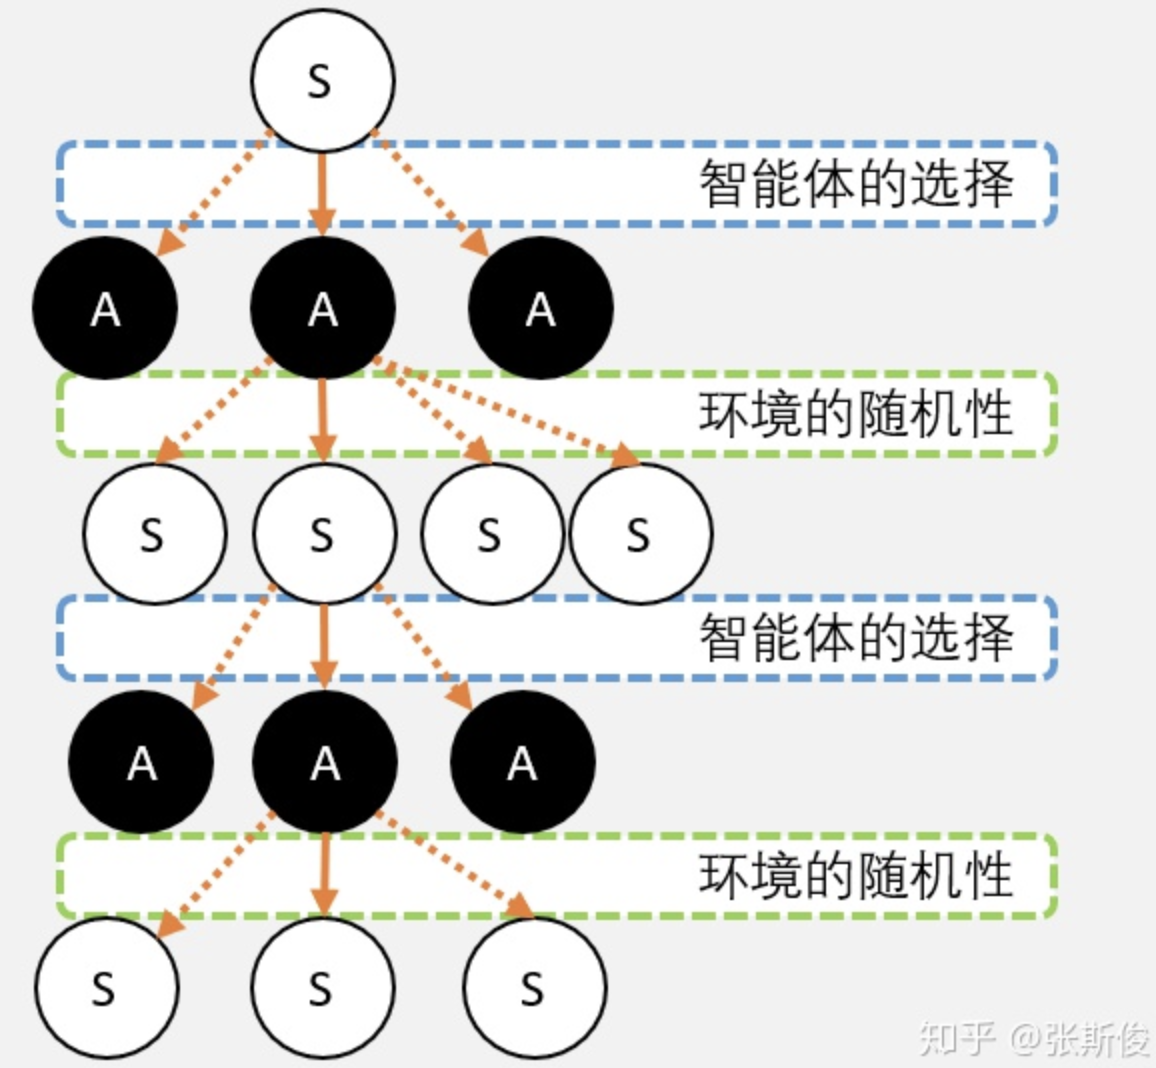
\includegraphics[width=.5\textwidth]{fig/ReinforcementLearning/RL_Markov_Chain_Tree_Uncertainty.png}
\end{figure}

\begin{framed}
\small{
举例:

假设现在我们来玩这样一个游戏。这个游戏是简化版的大富翁,我们只考虑我们当前所处位置,也就是状态。智能体移动的时候,它可以选择投掷\textbf{1-3个}骰子,根据骰子点数的总和向前移动。

现在,智能体从格子A掷骰子,并移动到格子B。其实经历了两次不确定性:(1)“选择”的过程。智能体主动选择骰子的个数。掷骰子的个数不同,到达格子B的概率也不同。所以“选择”会影响到下一个状态。这种不同动作之间的选择,我们称为智能体的策略。策略我们一般用Pi表示。我们的任务就是找到一个策略,能够获得最多的奖励;(2)环境的随机性,这是智能体无法控制的。在这个例子里就是骰子的随机性。注意,并不是所有环境都有随机性,有些环境是很确定的(例如把以上所有骰子每一面都涂成1点),但马尔科夫链允许我们有不确定性的存在。

也就是说,\textbf{虽然智能体不能控制环境的随机性,但能控制策略的选择,让智能体避免高风险低回报的情况出现}。
}
\end{framed}

\section{衡量节点的价值-V值和Q值\cite{How_To_Understand_Q_V_Value}}
\subsection{Q和V介绍}
于是,我们如果要想让智能体能够获得\textbf{奖励最大化},就面临两个问题:(1)未来的路很长,我们不能只凭眼前的收获,就马上做决定;我们要考虑未来;(2)未来的路充满不确定性:我们不能走一次某一条路,就下决定了。

那我们该怎么办呢?我们需要V和Q。\textbf{V是对状态节点的估算,Q是对动作节点的估算}。估算从该节点,一直到最终状态,能够获得的奖励的总和的平均值。也就是说,Q值和V值的概念是一致的,都是衡量在马可洛夫树上某一个节点的价值。只不过V值衡量的是状态节点的价值,而Q值衡量的是动作节点的价值。
\begin{figure}[H]
    \centering
    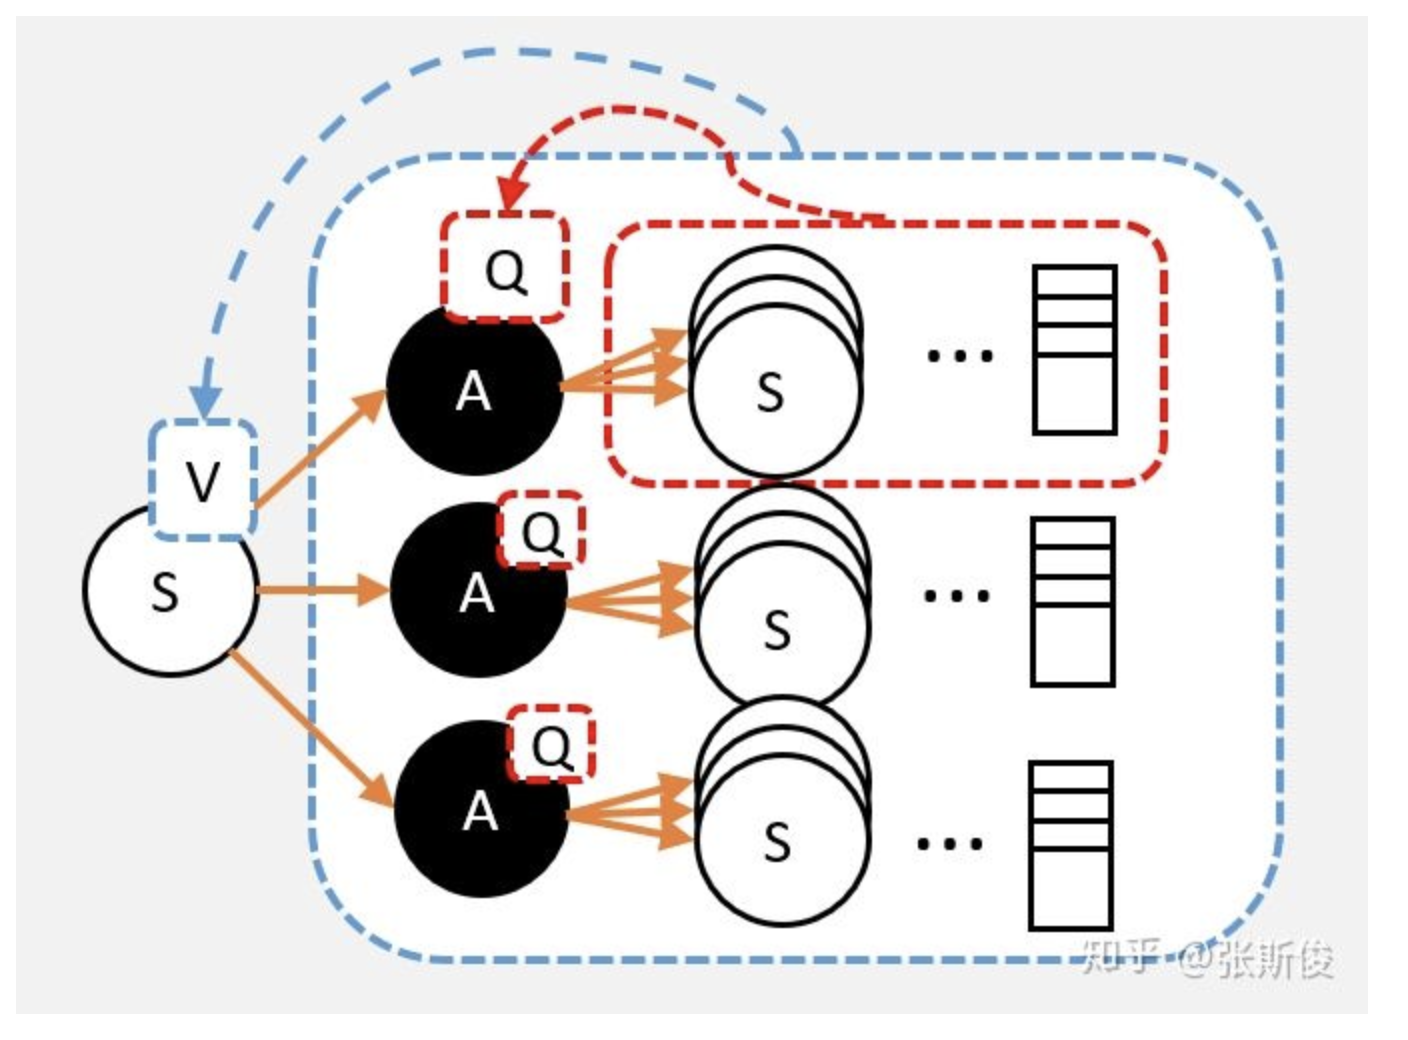
\includegraphics[width=.5\textwidth]{fig/ReinforcementLearning/RL_V_Q_Estimation.png}
\end{figure}

\begin{framed}
\small{
举例:
\begin{figure}[H]
    \centering
    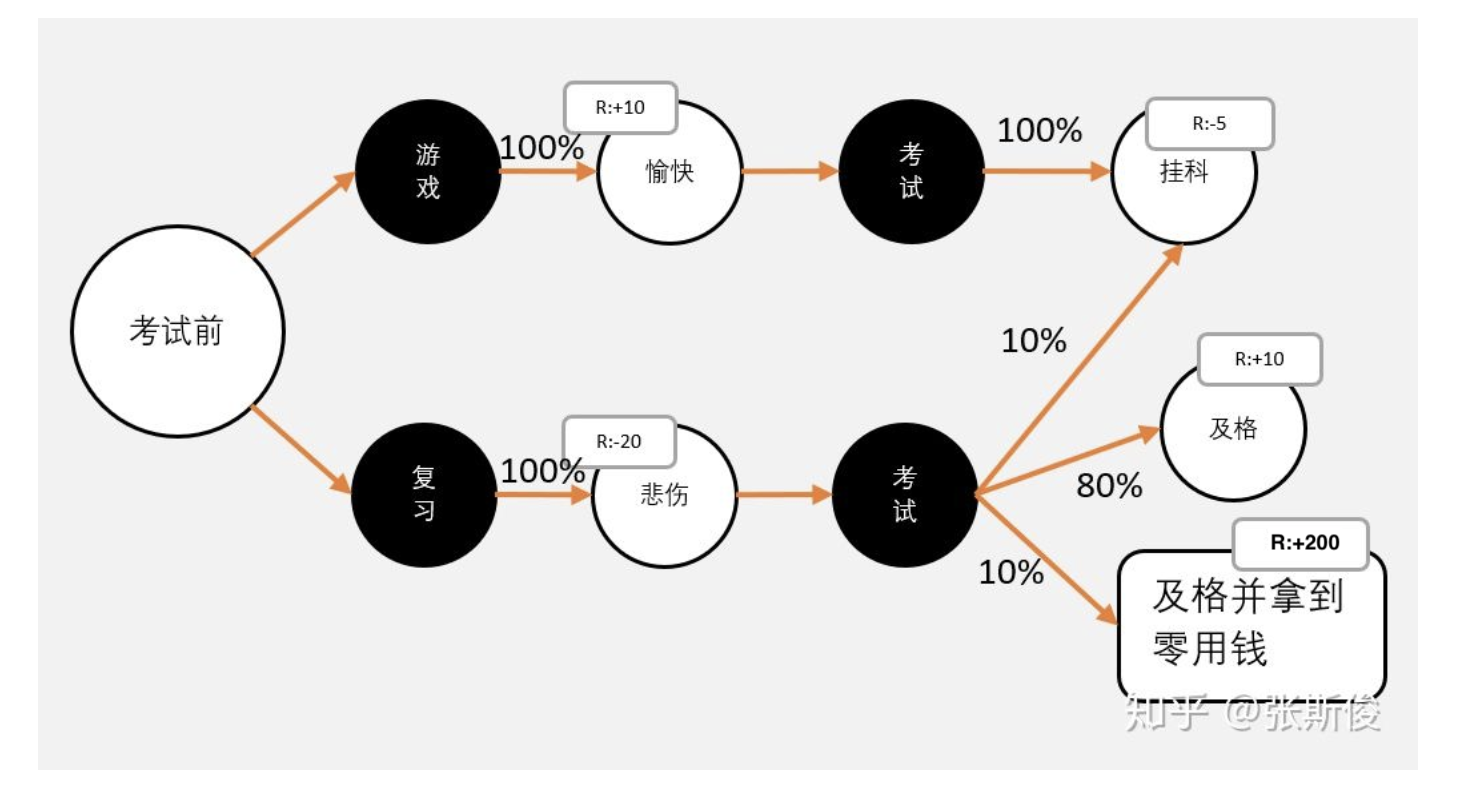
\includegraphics[width=1\textwidth]{fig/ReinforcementLearning/RL_V_Q_R_Example_1.png}
\end{figure}
\begin{figure}[H]
    \centering
    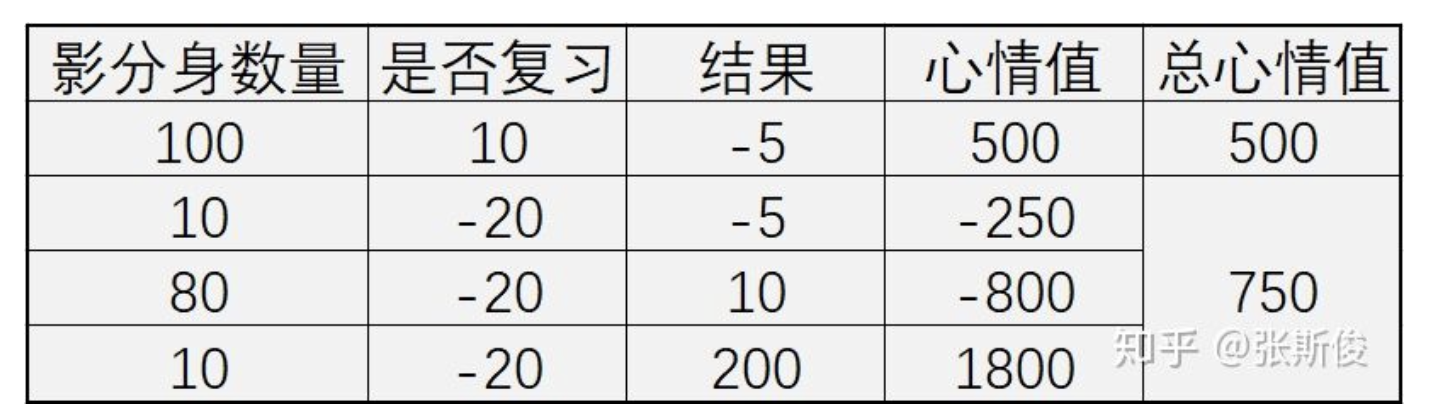
\includegraphics[width=.8\textwidth]{fig/ReinforcementLearning/RL_V_Q_R_Example_2.png}
\end{figure}
}
\end{framed}

看了上面的例子,感觉就是根据概率求期望;但在实际运用中,大多时候我们并不知道真实概率是多少。以上的概率都是我们自己估算,没有经过验证的。\textbf{在强化学习中,我们为了获得概率,我们将会不断地让我们智能体重复,或者让多个智能体进行试验以获得数据}。

\subsection{Q和V的意义}
智能体在做决策的时候,需要把眼光放远点,把未来的价值换到当前,才能做出选择。为了方便,我们希望可以有一种方法衡量我做出每种选择的价值。这样,我只要看一下标记,以后的事情我也不用理了,我选择那个动作价值更大,就选那个动作就可以了。

也就是说,在上面的例子中,我们让复习和游戏都有一个标记,这个标记描述了这个动作的价值: 游戏 +500;复习 +750;这面这个图是将标记表在了动作节点上:
\begin{figure}[H]
    \centering
    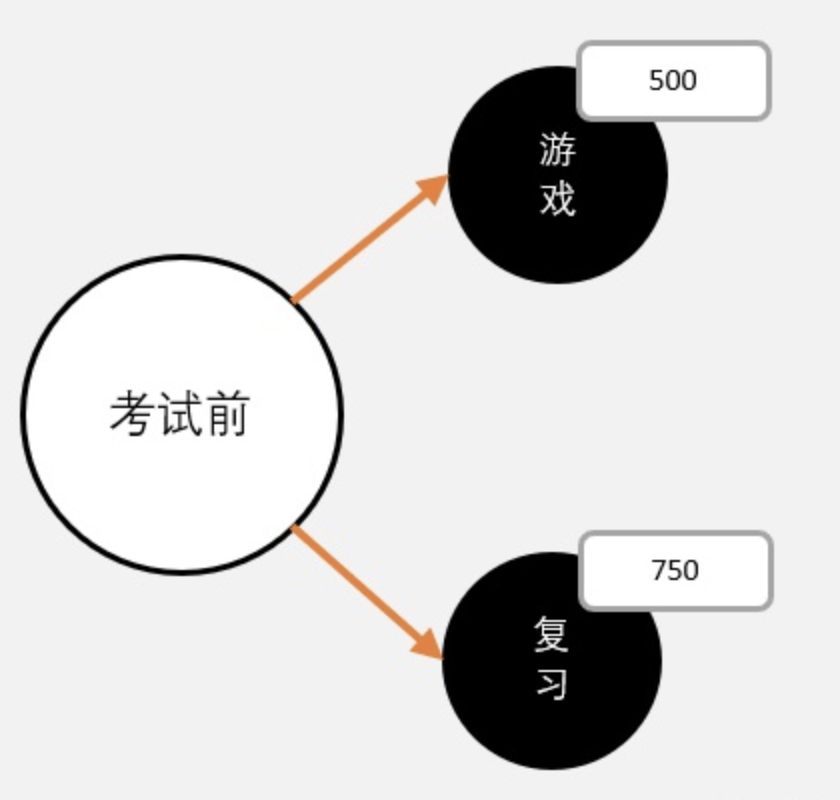
\includegraphics[width=.3\textwidth]{fig/ReinforcementLearning/RL_V_Q_R_Example_3.png}
\end{figure}

当然,我们也可以把这个标记标在状态节点上。为了方便沟通,我们这样定义: 
\begin{itemize}
\setlength{\itemsep}{0pt}
\setlength{\parsep}{0pt}
\setlength{\parskip}{0pt}
    \item 评估动作的价值,我们称为Q值:它代表了智能体选择这个动作后,一直到最终状态奖励总和的期望;
    \item 评估状态的价值,我们称为V值:它代表了智能体在这个状态下,一直到最终状态的奖励总和的期望。
\end{itemize}

价值越高,表示我从当前状态到最终状态能获得的平均奖励将会越高。因为智能体的目标数是获取尽可能多的奖励,所以智能体在当前状态,只需要选择价值高的动作就可以了。

\subsection{V值的定义}
假设现在需要求某状态S的V值,那么我们可以这样:
\begin{enumerate}
\setlength{\itemsep}{0pt}
\setlength{\parsep}{0pt}
\setlength{\parskip}{0pt}
    \item 我们从S点出发,并影分身出若干个自己;
    \item 每个分身按照当前的策略 选择行为;
    \item 每个分身一直走到最终状态,并计算一路上获得的所有奖励总和;
    \item 我们计算每个影分身获得的平均值,这个平均值就是我们要求的V值。
\end{enumerate}
\begin{figure}[H]
    \centering
    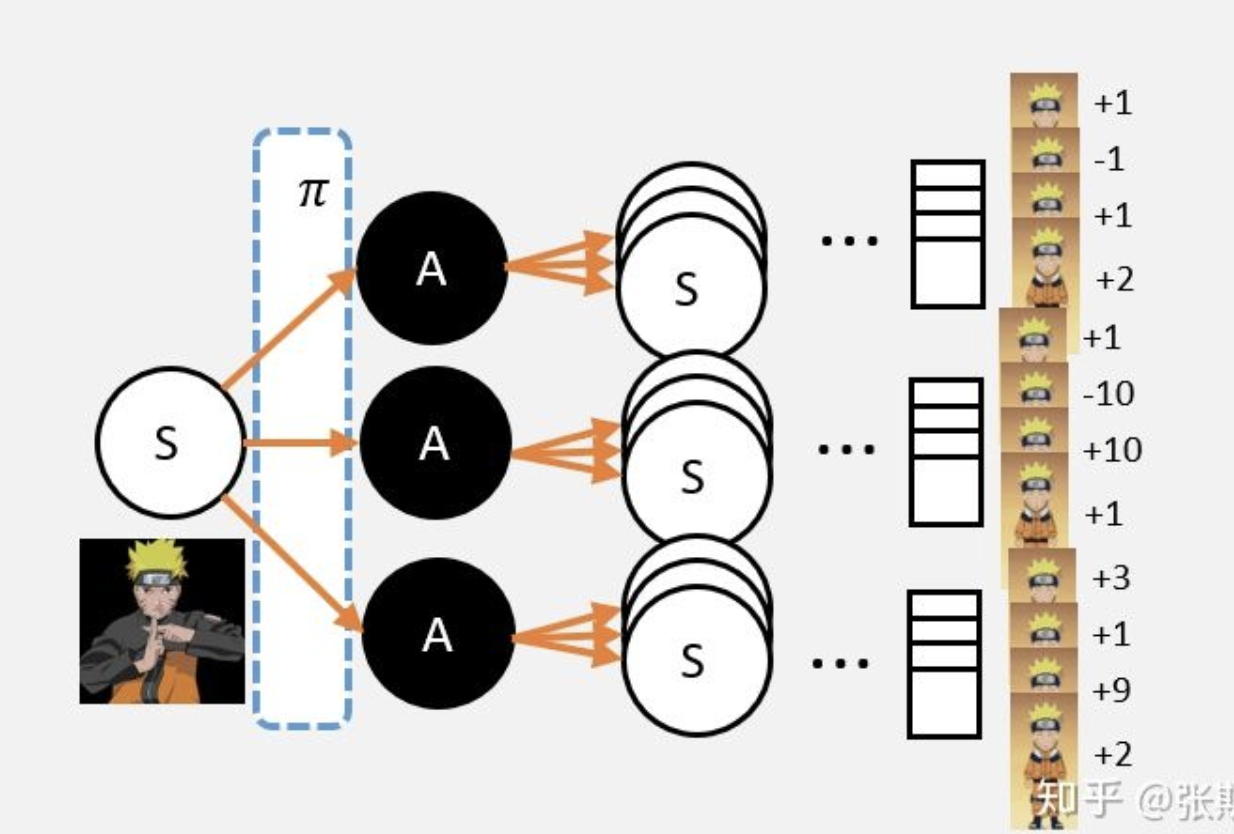
\includegraphics[width=.3\textwidth]{fig/ReinforcementLearning/RL_Compute_V.png}
\end{figure}

\begin{framed}
理解:

1. 从V值的计算,我们可以知道,V值代表了这个状态的今后能获得奖励的期望。从这个状态出发,到达最终状态,平均而言能拿到多少奖励。所以我们轻易比较两个状态的价值。

2. V值跟我们选择的策略有很大的关系。 我们看一个简化的例子,从S出发,只有两种选择,A1,A2;从A1,A2只有一条路径到最终状态,获得总奖励分别为10和20。

现在我们假设策略 采用平均策略$[A_1: \pi_1 = 50\%,A_2:\pi_2 = 50\%]$,根据用影分身,那么我们可以求得V值为$V_\pi = 0.5 \times 10 + 0.5 \times 20 = 15$;

现在我们改变策略$[A_1: \pi_1 = 60\%,A_2:\pi_2 = 40\%]$,那么我们可以求得V值为$V_\pi = 14$,变少了!

所以可以看出,\textbf{V值是会根据不同的策略而有所变化的}!
\end{framed}

\subsection{Q值的定义}
Q值和V值的概念是一致的,都是衡量在马可洛夫树上某一个节点的价值。只不过V值衡量的是状态节点的价值,而Q值衡量的是动作节点的价值。

现在我们需要计算,某个状态S0下的一个动作A的Q值:\begin{enumerate}
\setlength{\itemsep}{0pt}
\setlength{\parsep}{0pt}
\setlength{\parskip}{0pt}
    \item 从A这个节点出发,使用影分身之术;
    \item 每个影分身走到最终状态,并记录所获得的奖励;
    \item 求取所有影分身获得奖励的平均值,这个平均值就是我们需要求的Q值。
\end{enumerate}

\begin{figure}[H]
    \centering
    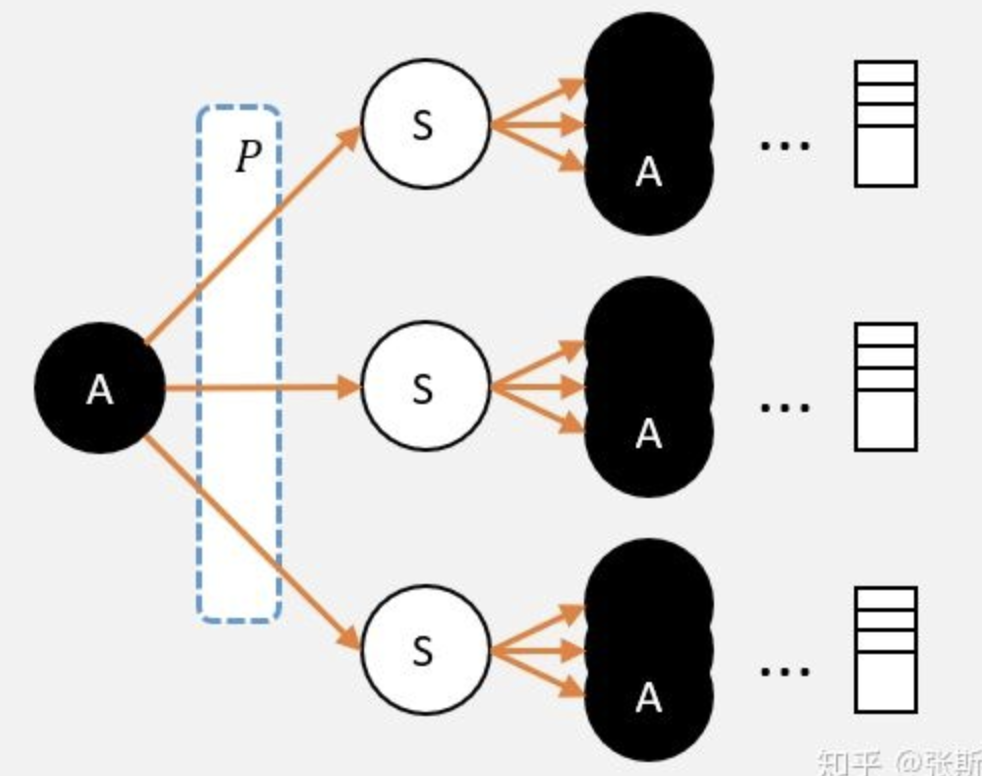
\includegraphics[width=.3\textwidth]{fig/ReinforcementLearning/RL_Compute_Q.png}
\end{figure}

\textbf{与V值不同,Q值和策略并没有直接相关,而与环境的状态转移概率相关,而}\textcolor{red}{环境的状态转移概率是不变的。}

\subsection{V值和Q值的关系}
从以上的定义,我们可以知道Q值和V值的意义相通的:
\begin{itemize}
\setlength{\itemsep}{0pt}
\setlength{\parsep}{0pt}
\setlength{\parskip}{0pt}
    \item 都是马可洛夫树上的节点;
    \item 价值评价的方式是一样的: 从当前节点出发;一直走到最终节点;所有的奖励的期望值
\end{itemize}

所以,\textbf{Q和V之间是可以相互换算的};

\subsubsection{从Q到V}
\begin{figure}[H]
    \centering
    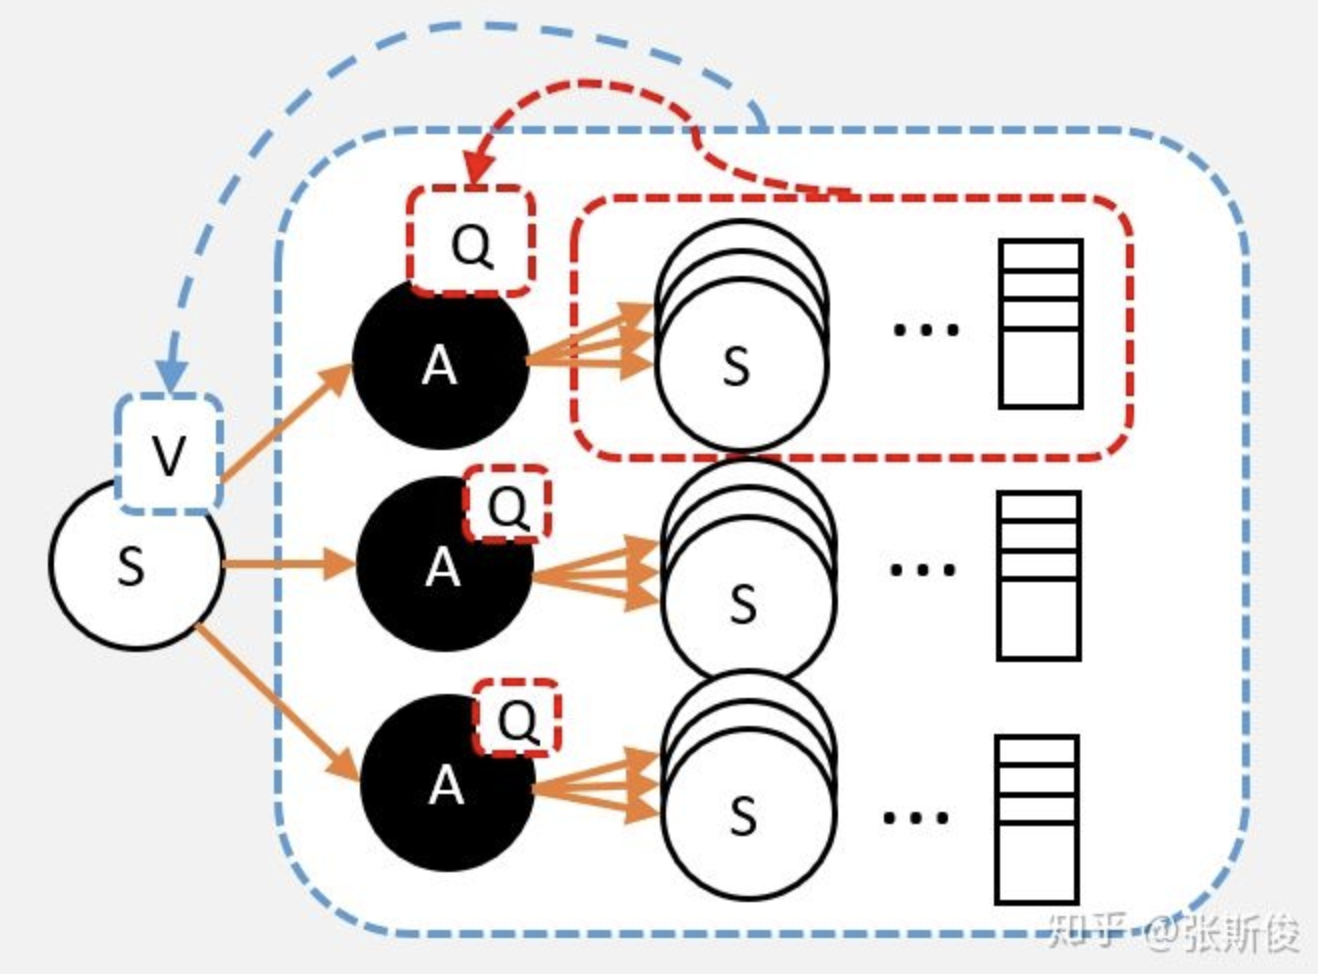
\includegraphics[width=.6\textwidth]{fig/ReinforcementLearning/RL_Compute_V_From_Q.png}
\end{figure}

从定义出发,我们要求的V值,就是从状态S出发,到最终获取的所获得的奖励总和的期望值。也就是蓝色框部分。

S状态下有若干个动作,每个动作的Q值,就是从这个动作之后所获得的奖励总和的期望值。也就是红色框部分。

假设我们已经计算出每个动作的Q值,那么在计算V值的时候就不需要一直走到最终状态了,只需要走到动作节点,看一下每个动作节点的Q值,根据策略 ,计算Q的期望就是V值了。

所以有如下V值的计算公式:
\begin{figure}[H]
    \centering
    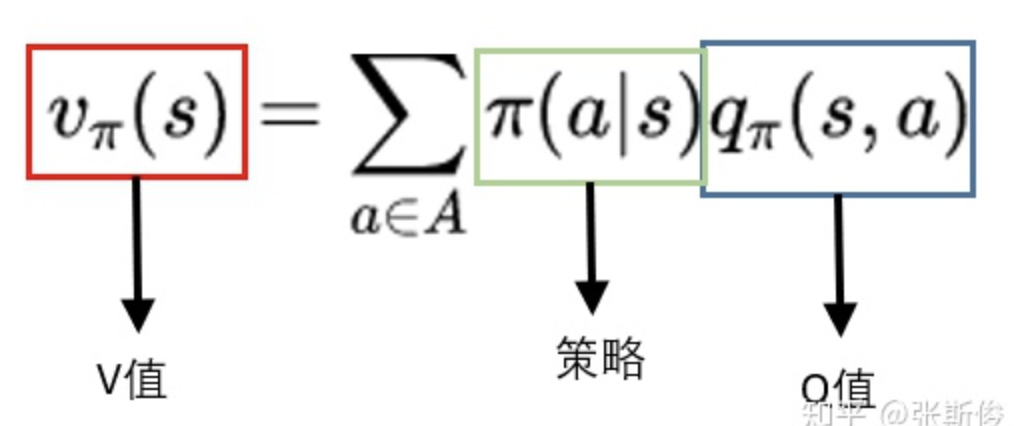
\includegraphics[width=.5\textwidth]{fig/ReinforcementLearning/RL_Compute_V_From_Q_Eq.png}
\end{figure}

\subsubsection{从V到Q}
道理还是一样,就是用Q就是V的期望!而且这里不需要关注策略,这里是环境的状态转移概率决定的。

但是需要注意的是,\textbf{当我们选择A,并转移到新的状态时,就能获得奖励,所以我们必须把这个奖励也算上!}
\begin{figure}[H]
    \centering
    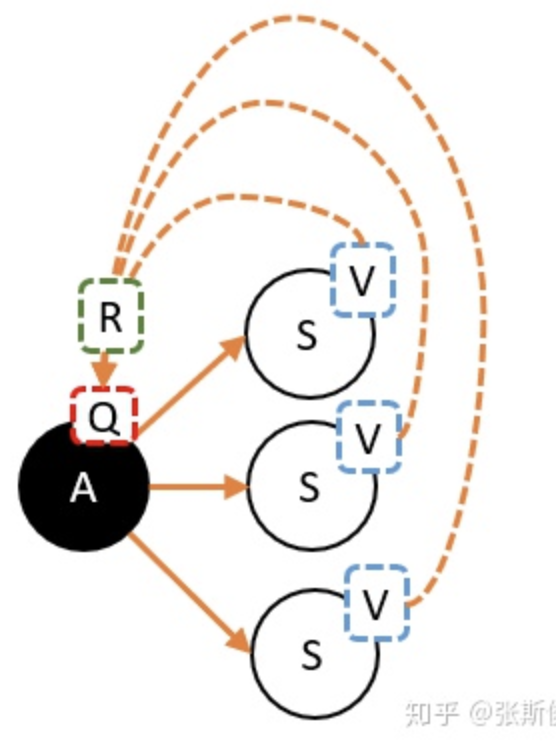
\includegraphics[width=.3\textwidth]{fig/ReinforcementLearning/RL_Compute_Q_From_V.png}
\end{figure}

所以有如下Q值的计算公式:
\begin{figure}[H]
    \centering
    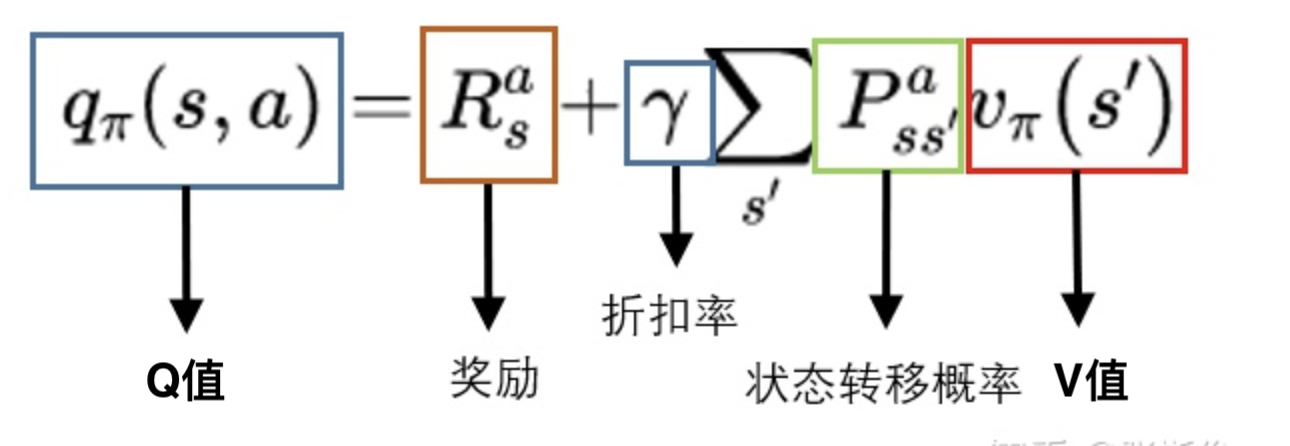
\includegraphics[width=.5\textwidth]{fig/ReinforcementLearning/RL_Compute_Q_From_V_Eq.png}
\end{figure}

\begin{framed}
\textbf{折扣率}:在强化学习中,有某些参数是人为主观制定。这些参数并不能推导,但在实际应用中却能解决问题,所以我们称这些参数为超参数,而折扣率就是一个超参数。 与金融产品说的贴现率是类似的。我们计算Q值,目的就是把未来很多步奖励,折算到当前节点。但未来n步的奖励的10点奖励,与当前的10点奖励是否完全等价呢?未必。所以我们人为地给未来的奖励一定的折扣,例如:0.9,0.8,然后在计算到当前的Q值。
\end{framed}

\subsubsection{从V到V}
从V到V也是很简单的。把公式代进去就可以了:
\begin{figure}[H]
    \centering
    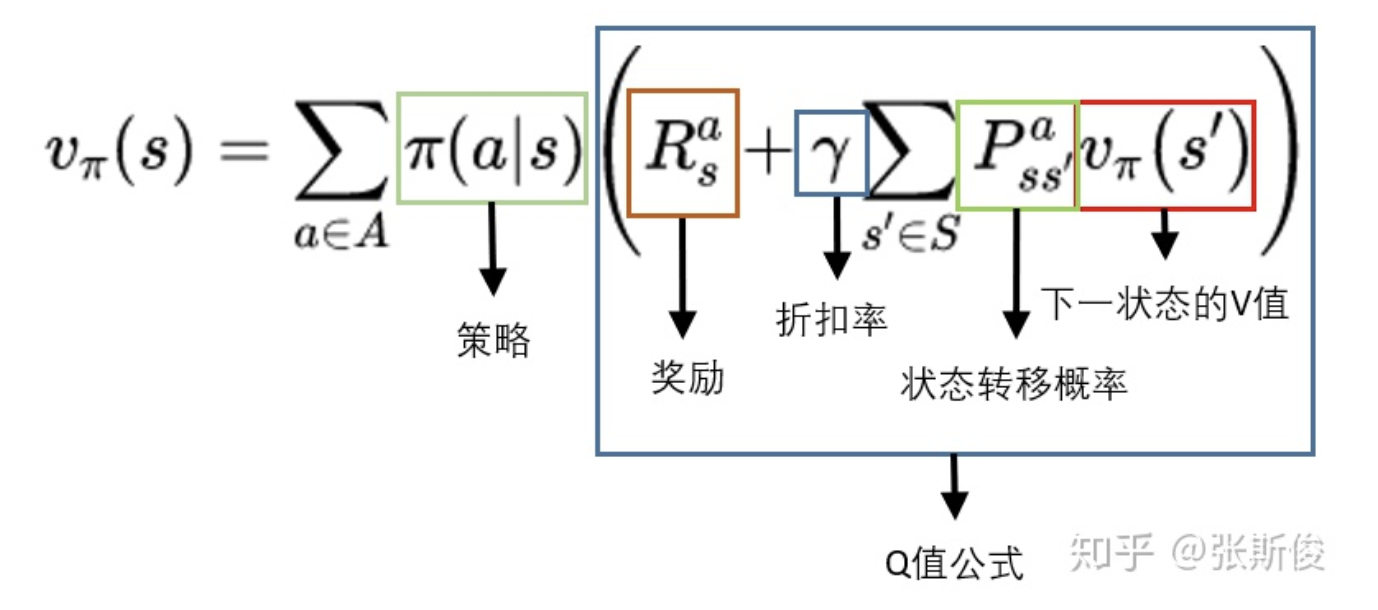
\includegraphics[width=.6\textwidth]{fig/ReinforcementLearning/RL_Compute_V_From_V_Eq.png}
\end{figure}

\subsection{Q值和V值的总结}
\begin{itemize}
\setlength{\itemsep}{0pt}
\setlength{\parsep}{0pt}
\setlength{\parskip}{0pt}
    \item V就是子节点的Q的期望,但要注意V值和策略相关;
    \item Q就是子节点的V的期望,但要注意,记得把R计算在内;
\end{itemize}

\section{估算节点的价值-蒙特卡洛(MC)和时序差分(TD)}
\subsection{蒙特卡洛MC}
那怎么估算每个节点的价值呢?蒙特卡洛会让智能体从某个状态S出发,直到最终状态,然后回过头来给每个节点标记这次的价值G。G代表了某次智能体在这个节点的价值。经过多次后,把每个状态的G值进行平均。这就是状态的V值。

\subsubsection{蒙特卡洛的具体算法}
\begin{enumerate}
\setlength{\itemsep}{0pt}
\setlength{\parsep}{0pt}
\setlength{\parskip}{0pt}
    \item 把智能体放到环境的任意状态;
    \item 从这个状态开始按照策略进行选择动作,并进入新的状态;
    \item 重复步骤2,直到最终状态;
    \item 我们从最终状态开始向前回溯:计算每个状态的G值;
    \item 从这个状态开始按照策略进行选择动作,并进入新的状态;
    \item 重复1-4多次,然后平均每个状态的G值,这就是我们需要求的V值;
\end{enumerate}

为了方便,我们对平均进行一些优化。于是获得用MC估算V值的公式:
\begin{figure}[H]
    \centering
    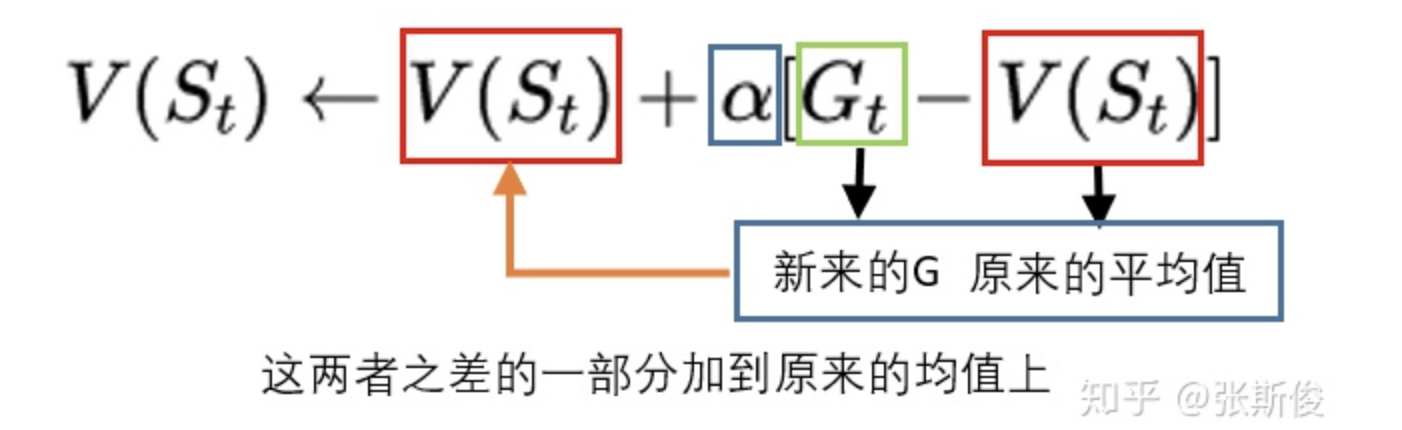
\includegraphics[width=.5\textwidth]{fig/ReinforcementLearning/RL_Compute_V_By_MC.png}
\end{figure}


\begin{framed}
理解用MC估算V值的公式:

V是G的平均值,但我们可以用\textbf{增量更新的方式}: 现在我们只需要记录之前的平均值V,新加进来的G,和次数N。我们把V和G的差,除以N,然后再加到原来的平均值V上,就能计算到新的V值。 即:V\_new = (V\_old - G) * (1 / N) + V\_old

V\_old:原来的V值; G:这一次回溯后,计算出来的G值;N: 这个状态被经过多少次了; V\_new:新计算出来的V值。

但其实这样计算还是比较麻烦,我们甚至可以不用记录N,把(1/N)设置成为一个固定的数,例如0.1、0.2,我们把这个值称为\textbf{学习率$\alpha$}。

因此,可以将上述公式类比为梯度下降的形式,\textbf{V的更新目标就是G}:
\begin{figure}[H]
    \centering
    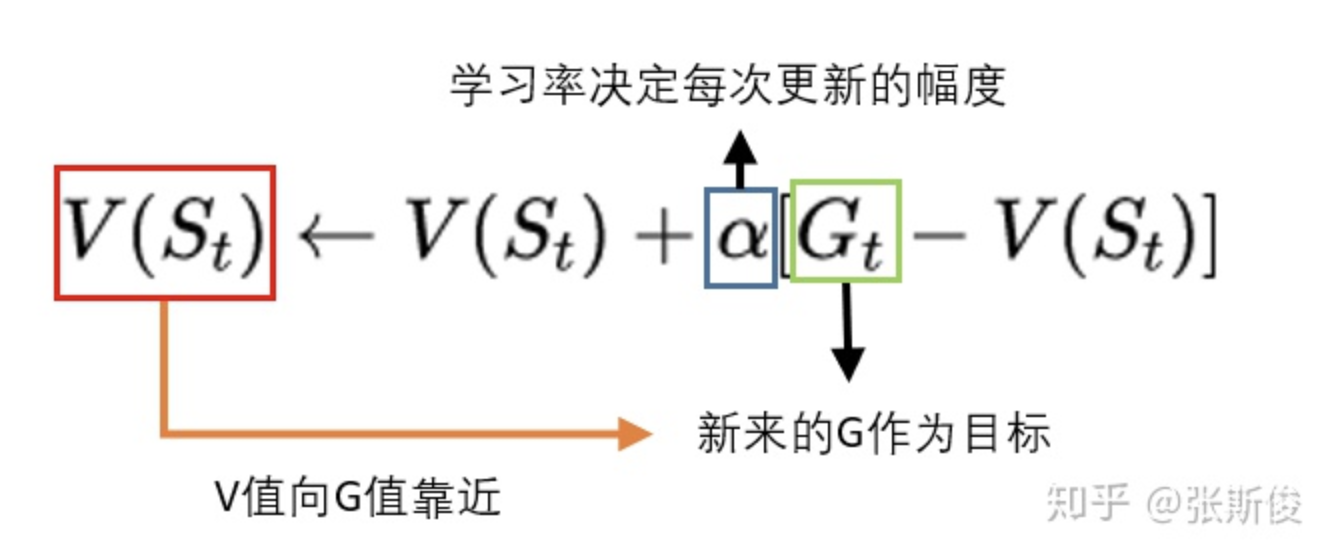
\includegraphics[width=.5\textwidth]{fig/ReinforcementLearning/RL_G_Meaning_5.png}
\end{figure}
\end{framed}

\begin{framed}
理解:\textbf{比较动态规划法和蒙特卡洛法}

动态规划方法,是\textbf{遍历了所有可能的情况},求得全局最优解;

蒙特卡洛法是进行了(放回)采样(允许重复),求得局部最优解;
\end{framed}

\subsubsection{蒙特卡洛的原理}
我们分成两部分,首先我们要理解每一次我们算的G值的意义。
\begin{figure}[H]
    \centering
    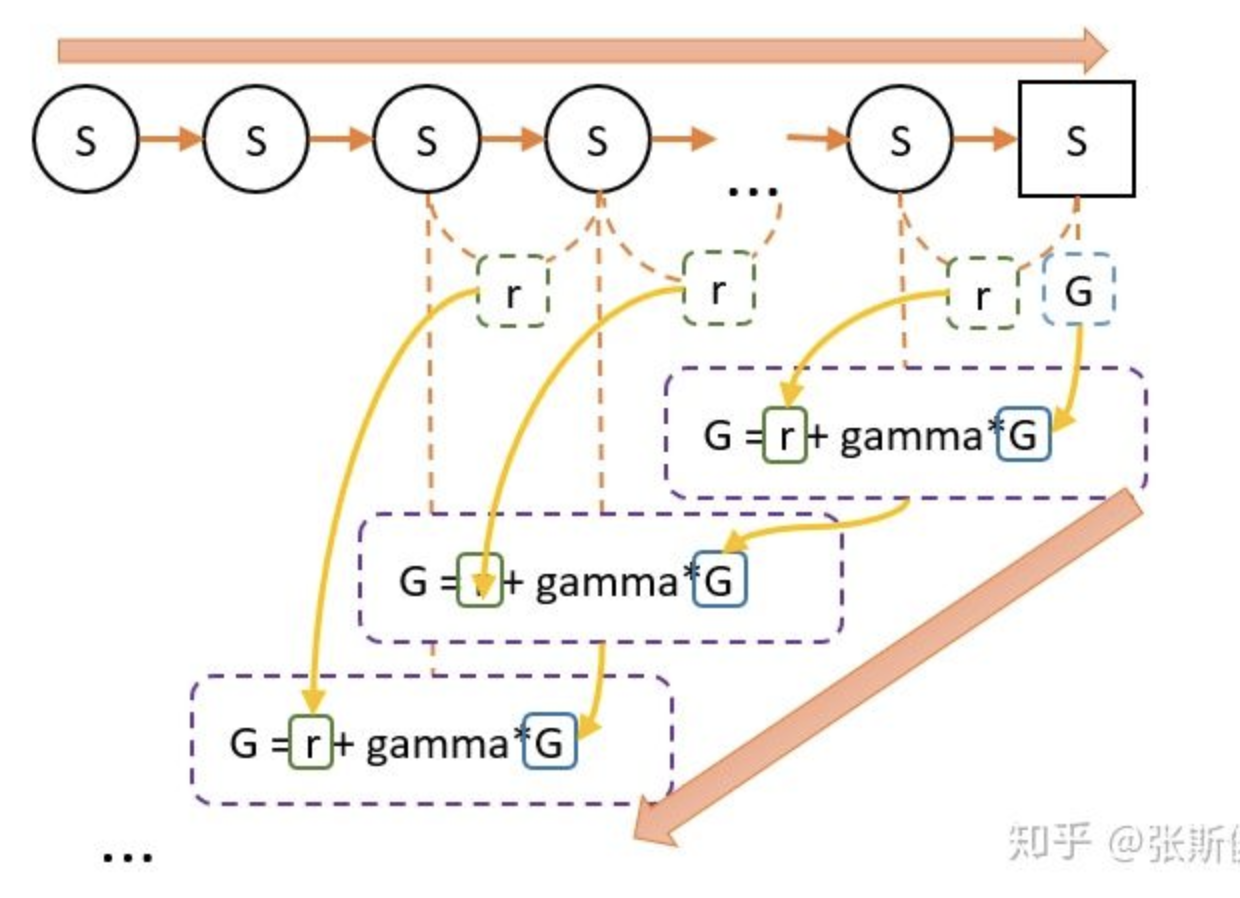
\includegraphics[width=.6\textwidth]{fig/ReinforcementLearning/RL_MC_Example.png}
\end{figure}

\begin{enumerate}
\setlength{\itemsep}{0pt}
\setlength{\parsep}{0pt}
\setlength{\parskip}{0pt}
    \item 我们根据策略往前走,一直走到最后,期间我们什么都不用算,还需要记录每一个状态转移,我们获得多少奖励r即可。;
    \item 我们从终点往前走,一遍走一遍计算G值。G值等于上一个状态的G值(记作G'),乘以一定的折扣(gamma),再加上r;
\end{enumerate}

所以G值的意义在于,在这一次游戏中,某个状态到最终状态的奖励总和(理解时可以忽略折扣值)
\begin{figure}[H]
    \centering
    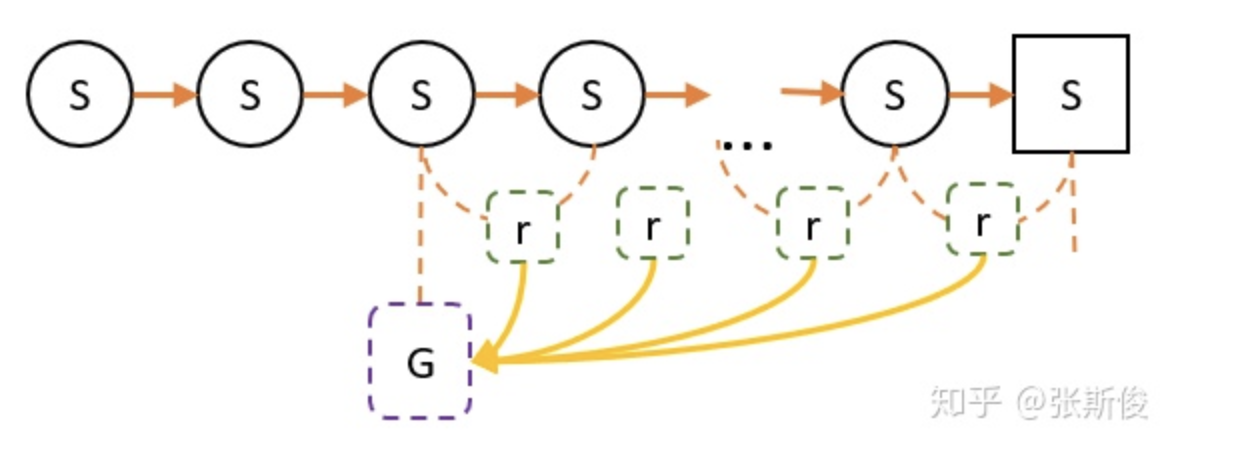
\includegraphics[width=.6\textwidth]{fig/ReinforcementLearning/RL_G_Meaning.png}
\end{figure}

当我们进行多次试验后,我们有可能会重复经过某个状态多次,通过回溯,也会有多个G值。 重复我们刚才说的,每一个G值,就是每次到最终状态获得的奖励总和。而V值是某个状态下,我们通过影分身到达最终状态,所有影分身获得的奖励的平均值。
\begin{figure}[H]
    \centering
    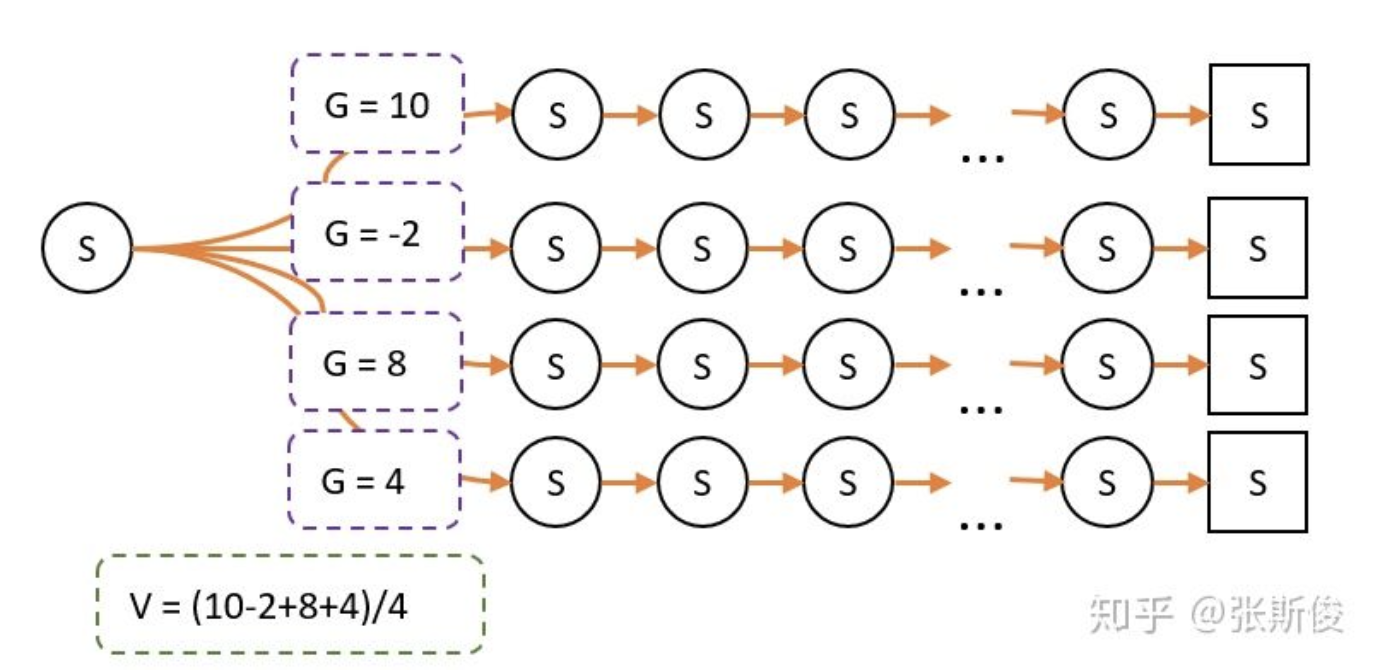
\includegraphics[width=.6\textwidth]{fig/ReinforcementLearning/RL_G_Meaning_2.png}
\end{figure}

\subsubsection{蒙特卡洛与策略选择的关系}
需要重点理解两点:\textbf{1. G的意义:在某个路径上,状态S到最终状态的总收获;2. V和G的关系:V是G的平均数。}

到这里要注意一点:V和策略是相关的,那么在这里怎么体现呢?这个非常重要,因为在PPO算法中,离线策略就与这个有关。这里可以稍微先说一下。我们仍以上图为例子,以平均策略A进行游戏。其中有100次经过S点,经过S点后有4条路径到达最终状态,计算G值和每条路径次数分别如下:
\begin{figure}[H]
    \centering
    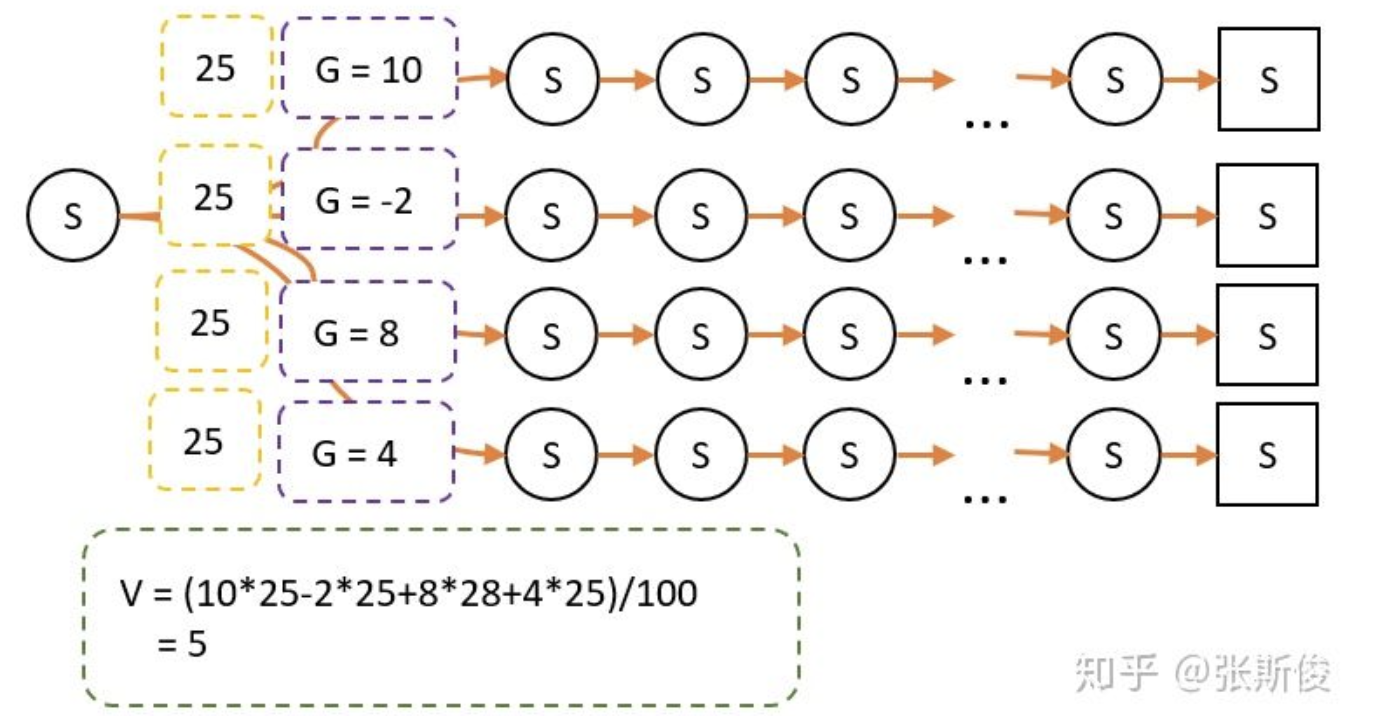
\includegraphics[width=.6\textwidth]{fig/ReinforcementLearning/RL_G_Meaning_3.png}
\end{figure}

策略A采用平均策略,这时候 V = 5。

现在我们采用策略B,\textbf{由于策略改变,经过某条路径的概率就会产生变化。因此最终试验经过的次数就不一样了}。
\begin{figure}[H]
    \centering
    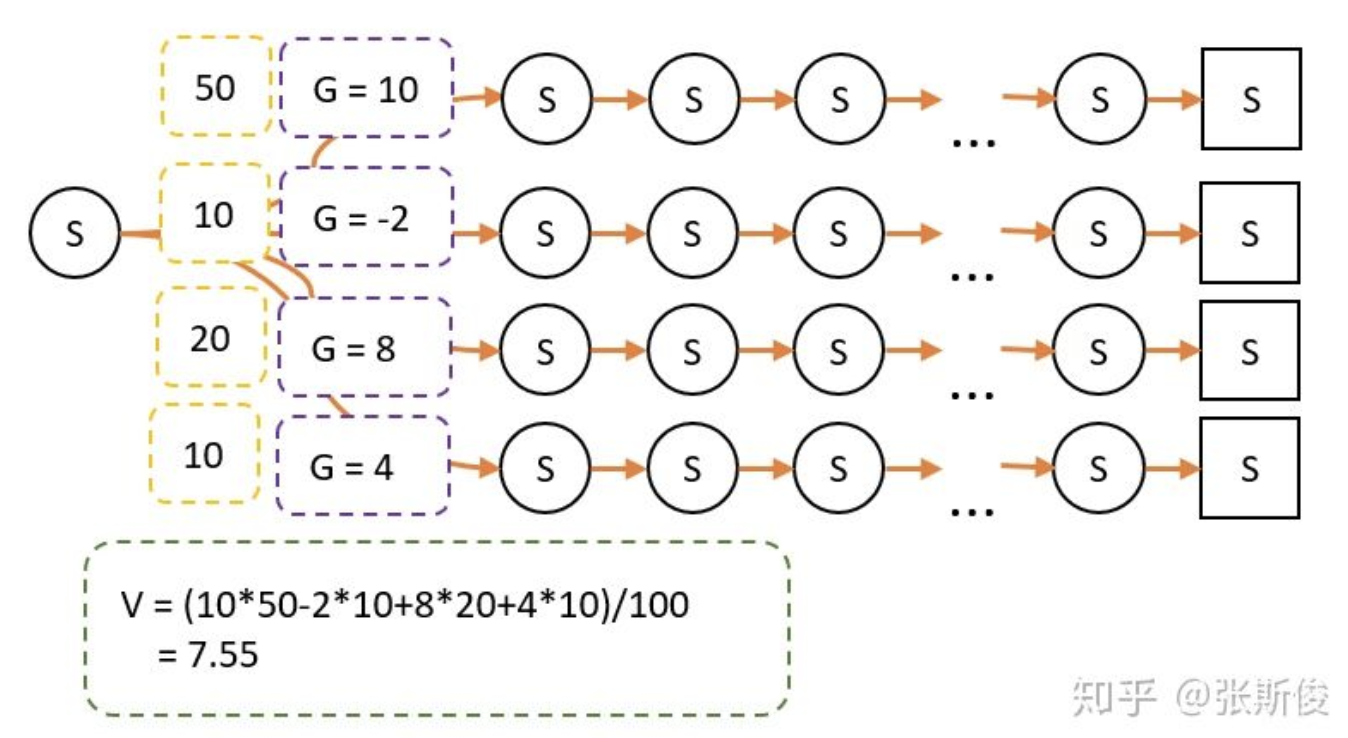
\includegraphics[width=.6\textwidth]{fig/ReinforcementLearning/RL_G_Meaning_4.png}
\end{figure}
策略B不是平均策略,最终计算的 V = 7.55。

\subsubsection{蒙特卡洛的缺陷}
在实际引用中,蒙特卡洛虽然比动态规划消耗要少一点;而且并不需要知道整个环境模型。但是它仍有一个比较大的缺点:就是每一次游戏,都需要先从头走到尾,再进行回溯更新。如果最终状态很难达到,或者环境的状态空间非常大,那可能每一次都要迭代很久能更新一次G值。

因此,蒙特卡洛算法单独拿出来,在强化学习中效率还是比较低的。所以会结合其他的方式进行应用。


\subsection{时序差分TD}
\subsubsection{时序差分算法原理}
蒙特卡洛每次估算G值都需要走到最终状态;而时序差分是一步一回头,用下一步的估值,估算当前状态的估值。
\begin{figure}[H]
    \centering
    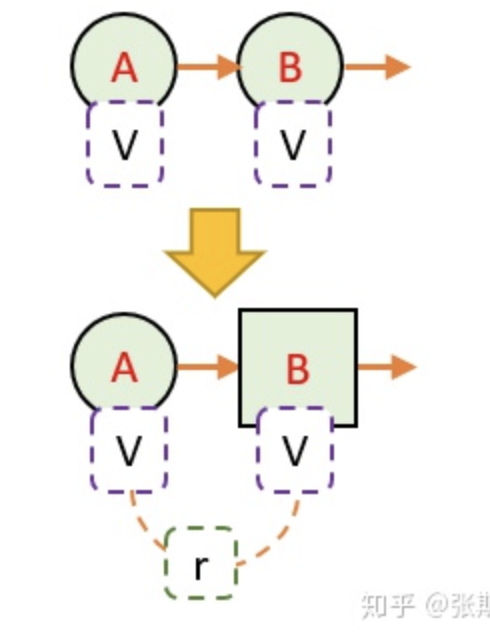
\includegraphics[width=.2\textwidth]{fig/ReinforcementLearning/RL_Compute_V_By_TD.png}
\end{figure}

这就相当于,把下一步状态直接当成最终状态。但这个状态它自己包含了这个状态的价值。因此,我们可以把蒙地卡罗用到的G值,用$V(S_{t+1})+ r$ 代 替。

\subsubsection{TD和MC的比较}
TD算法对MC进行了改进:
\begin{enumerate}
\setlength{\itemsep}{0pt}
\setlength{\parsep}{0pt}
\setlength{\parskip}{0pt}
    \item 和 MC 不同:TD 算法只需要走 N 步。就可以开始回溯更新;
    \item 和 MC 一样:需要先走 N 步,每经过一个状态,把奖励记录下来。然后开始回溯;
    \item 那么,状态的V值怎么算呢?其实和 MC 一样,我们就假设 N 步之后,就到达了最终状态了;假设“最终状态”上我们之前没有走过,所以这个状态上的值是空白的,这个时候我们就当这个状态为0;- 假设“最终状态”上我们已经走过了,这个状态的V值,就是当前值。然后我们开始回溯。
\end{enumerate}

\subsubsection{TD原理的直观理解}
我们可以把TD看成是这样一种情况:我们从A状态,经过1步,到B状态。我们什么都不管就当B状态是最终状态了。但B状态本身就带有一定的价值,也就是V值。其意义就是从B状态到最终状态的总价值期望。我们假设B状态的V值是对的,那么,通过回溯计算,我们就能知道A状态的更新目标了。

这就有点像从山顶像知道要下山的路有多长。 MC能直接走一趟,看一下到底有多远。 TD则轻巧一点,先走一段路看一下,看一下有没有路牌指示到山脚还有多远。如果有,那么就把刚刚走的那段路加上路牌指示到山脚的距离相加即可。 但又同学可能会问,在一开始,我们根本没有路牌呀,所以也不知道到底到山脚有多远。 没错,这是对的。但当我们走很多次的时候,路牌系统就能慢慢建立起来。 例如第一次,只有到了山脚,我才知道山脚前一站离山脚的的真实距离。于是我更新了山脚前一站的路牌。第二次,我在山脚前一站路就能看到路牌,所以我就可以更新山脚前一站的路牌了...一直到山顶,就这样一直建立整座山的路牌系统。

\subsubsection{TD算法的更新公式}
刚刚我们对TD有个直观的理解:TD并走走完整段路程,而是半路就截断。用半路的路牌,更新当前的路牌。

所以我们只需要把MC的更新目标,改为TD的更新目标即可。

\textbf{在MC,G是更新目标,而在TD,我们只不过把更新目标从G,改成r+gamma*V}:
\begin{figure}[H]
    \centering
    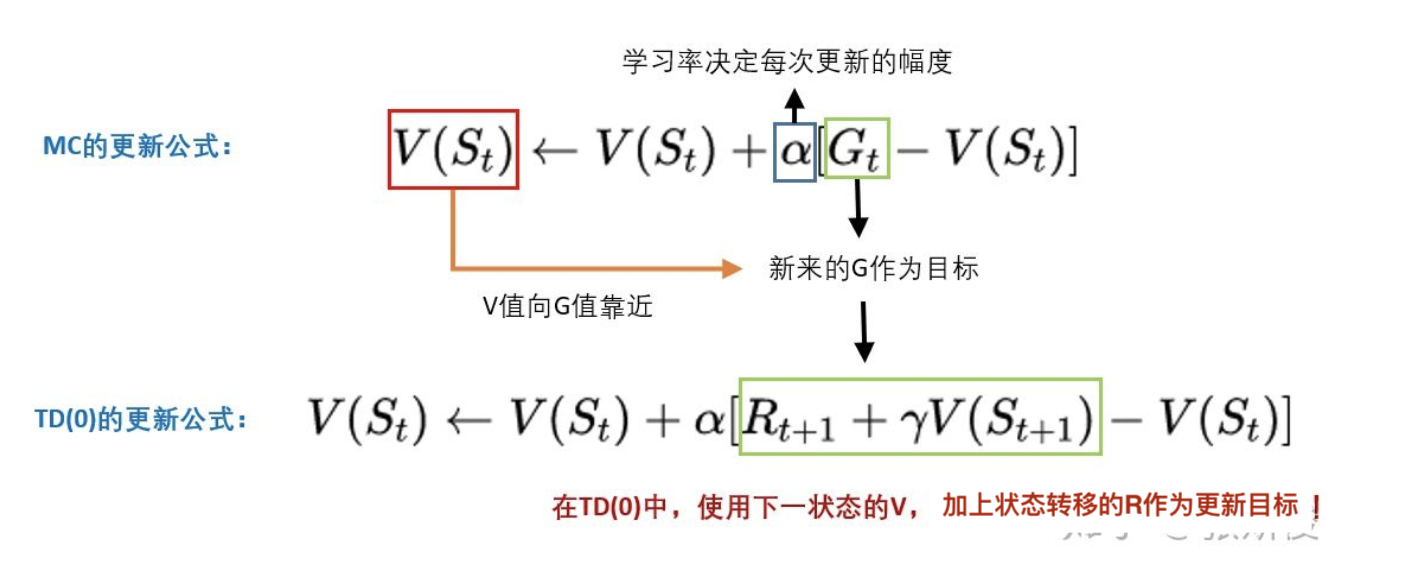
\includegraphics[width=1\textwidth]{fig/ReinforcementLearning/RL_Compute_V_By_TD_MC_Compare.png}
\end{figure}

\section{QLearning 和 SARSA}
我们之前学习了用TD估算V值。但其实我们用TD预估Q值,其实会来得更方便,因为我们要的就是智能体选择动作嘛。
\begin{figure}[H]
    \centering
    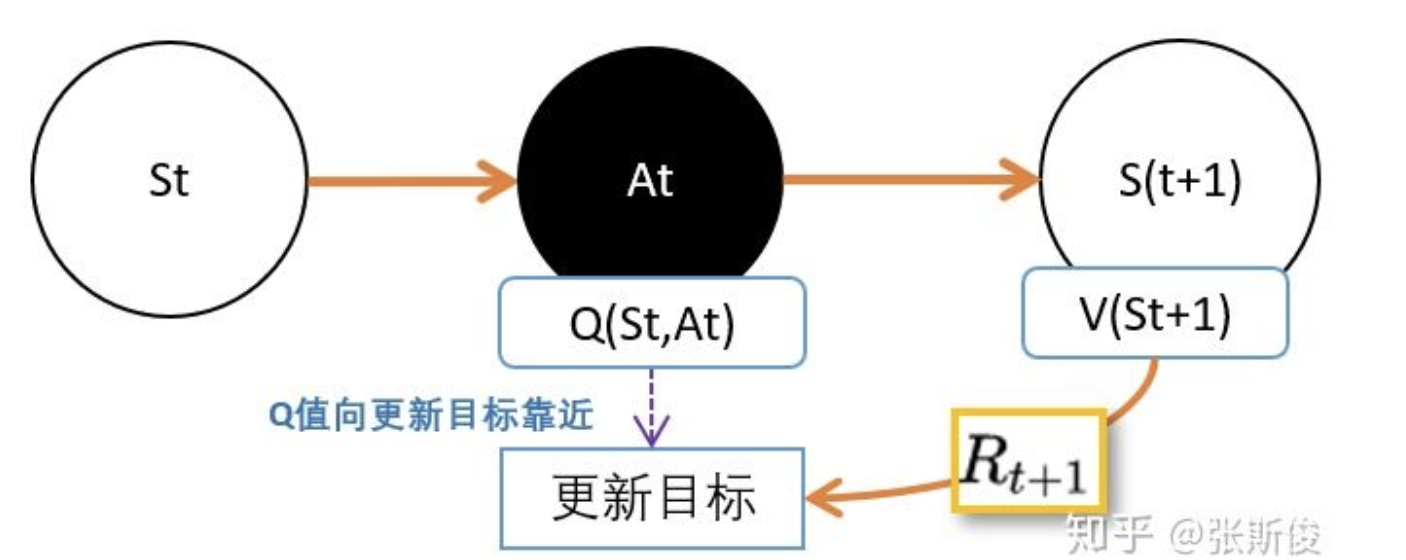
\includegraphics[width=.8\textwidth]{fig/ReinforcementLearning/RL_TD_For_Q.png}
\end{figure}

但问题是,如果既要估算$V(S_{t+1})$,又要估算$Q(S_t,A_t)$,就相当麻烦了。能不能都统一成Q值呢?也就是说$V(S_{t+1})$用一个动作的Q值所代替。\textbf{于是便有两种不同的替代方案:Qlearning和SARSA。}

\subsection{SARSA}
SARSA的想法是,用\textbf{同一个策略下产生的动作A的Q值替代;也就是说,St选At的策略和St+1选At+1是同一个策略。
$V(S_{t+1})$}。
\begin{figure}[H]
    \centering
    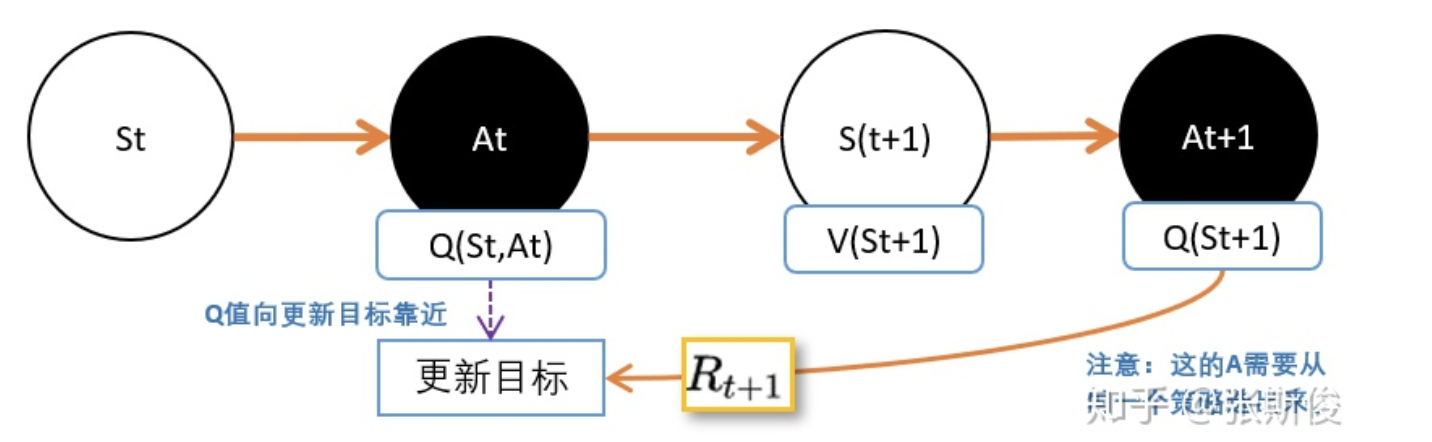
\includegraphics[width=.8\textwidth]{fig/ReinforcementLearning/RL_SARSA_Update_V.png}
\end{figure}

于是有了,SARSA的更新公式:
\begin{figure}[H]
    \centering
    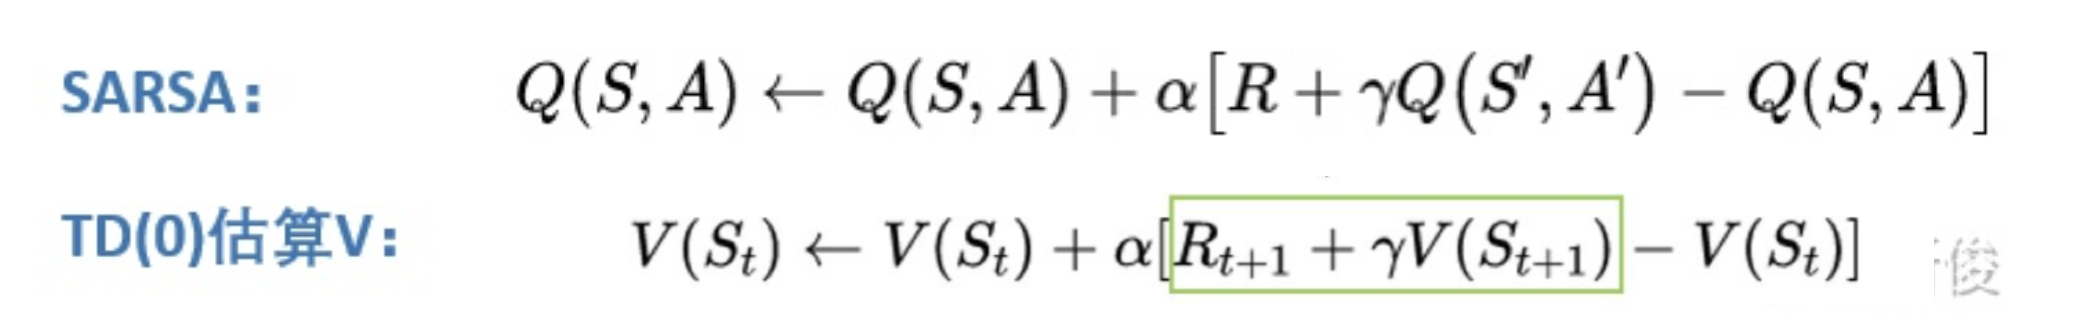
\includegraphics[width=.8\textwidth]{fig/ReinforcementLearning/RL_SARSA_Update_V_Eq.png}
\end{figure}

我们可以和TD估算V值对比一下,几乎是一模一样的,只是把V换成Q。但我还是建议记得我们上面说的,我们有用Q替代V(St+1)。因为跳过这一步,我们就理解不了QLearning了。

\subsection{QLearning}
QLearning 的想法其实也很直观:既然我们的目标是选取最大收益,所以,我们肯定会选择一个能够获得最大 Q 值的动作。也就是说,在实际选择中,我不可能选择不是最大 Q 值的动作。所以,我们应该用所有动作的Q值的最大值替代 $V(S_{t+1}) $。
\begin{figure}[H]
    \centering
    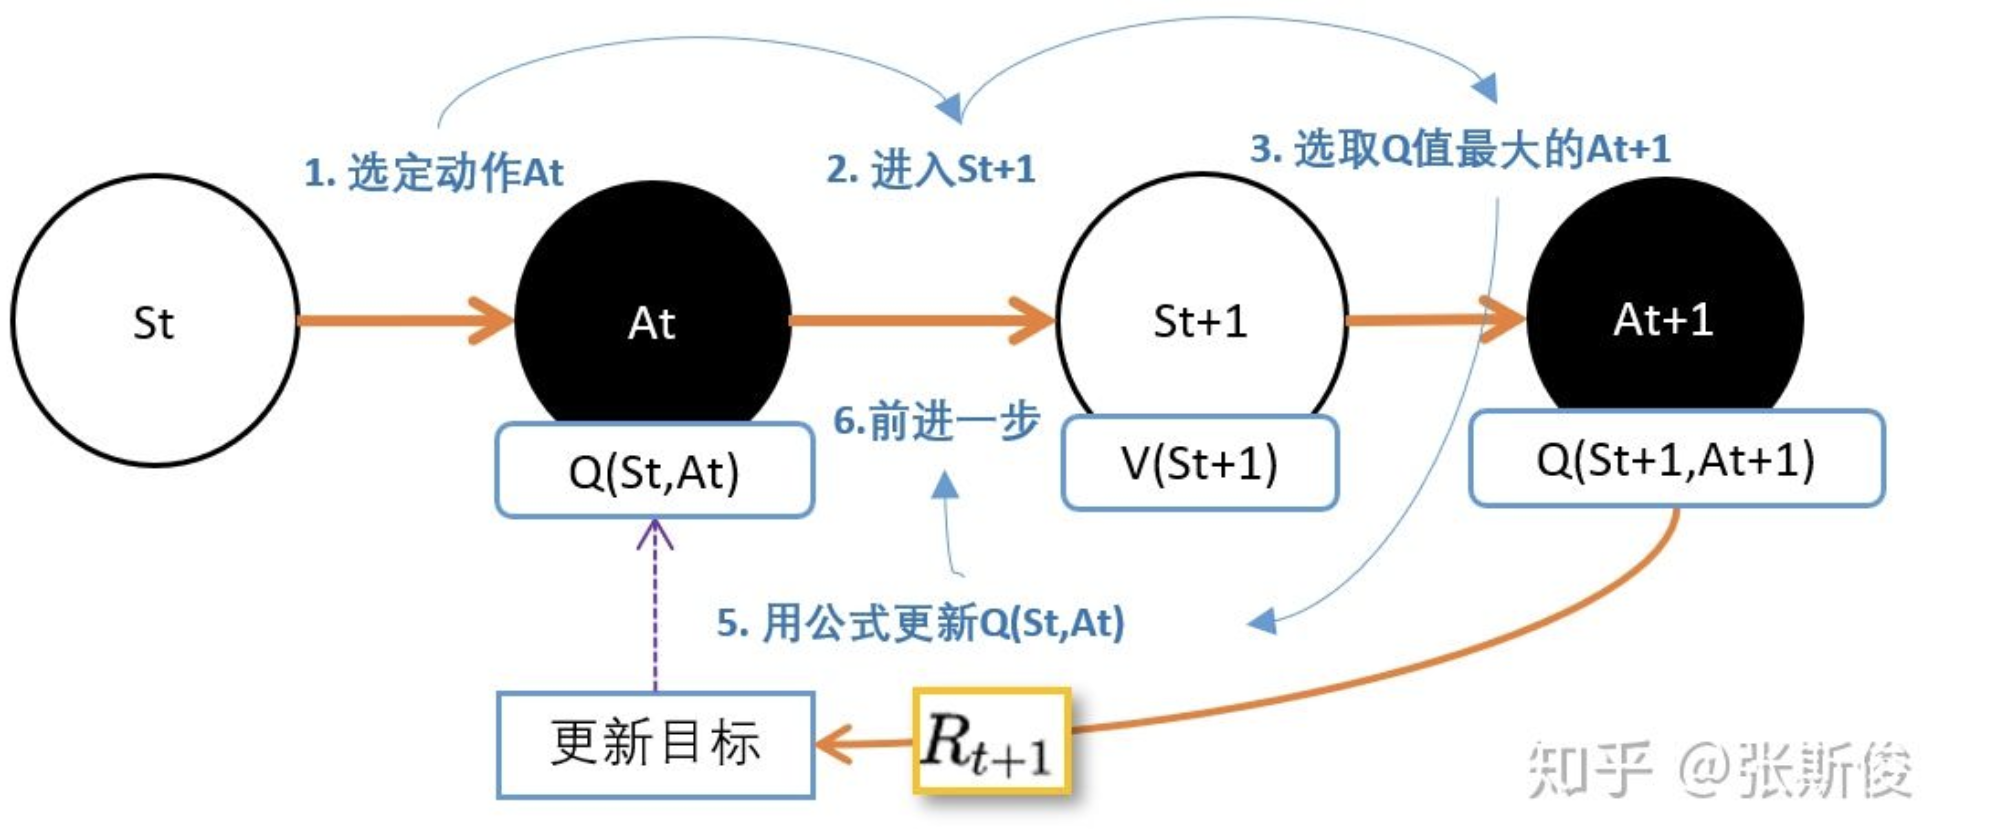
\includegraphics[width=.8\textwidth]{fig/ReinforcementLearning/RL_QLearning_Update_V.png}
\end{figure}

从马尔科夫树的角度来看,有下图:
\begin{figure}[H]
    \centering
    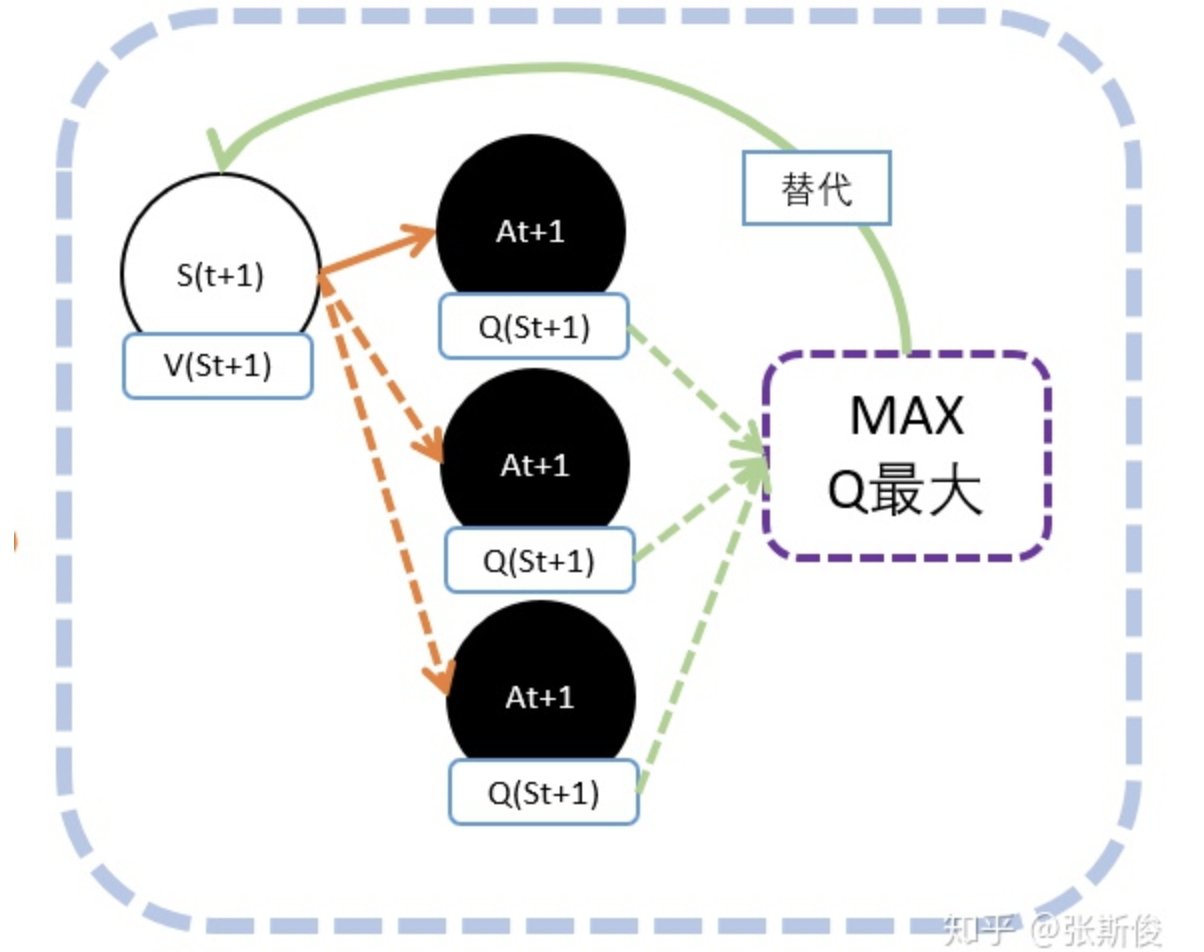
\includegraphics[width=.6\textwidth]{fig/ReinforcementLearning/RL_QLearning_Select_Max.png}
\end{figure}

所以我们就有了 QLearning 的更新公式:
\begin{figure}[H]
    \centering
    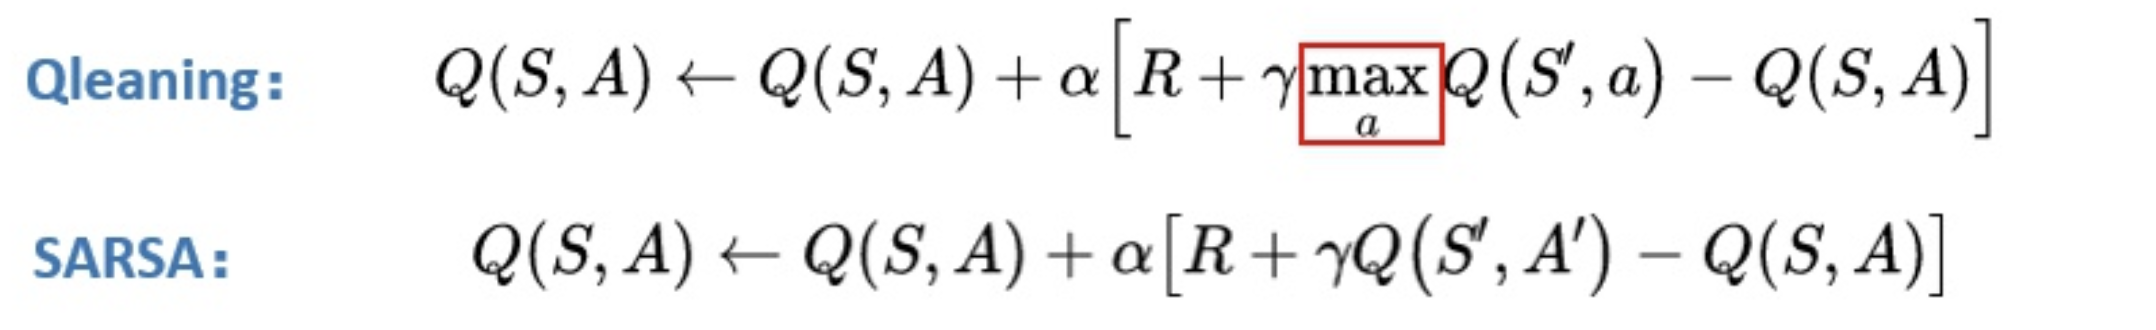
\includegraphics[width=.8\textwidth]{fig/ReinforcementLearning/RL_QLearning_Update_V_Eq.png}
\end{figure}

\subsection{QLearning和SARSA比较}
QLearning 公式和 SARSA 相比,就差那么一个 max:

(1)在相同策略下产生的动作 At+1。这就是 SARSA。也就是说,St 选 At的策略和 St+1 选 At+1 是同一个策略。

(2)选择能够产生最大 Q 值的动作 At+1。这就是 Qlearning。 Qlearning  能够产生最大 Q 值的动作 At+1 的 Q 值作为 V(St+1) 的替代。

\subsection{QLearning 算法流程\cite{Implement_QLearning}}
先总结下 QLeanring 的更新流程。 我们将会在任意的state出发:
\begin{enumerate}
\setlength{\itemsep}{0pt}
\setlength{\parsep}{0pt}
\setlength{\parskip}{0pt}
    \item 会用 noisy-greedy 的策略选定动作A;
    \item 在完成动作后,我将会进入新状态$S_{t+1}$;
    \item 检查 $S_{t+1}$ 中所有动作,看看哪个动作的Q值最大;
    \item 更新当前动作 A 的 Q 值:
    $$
    Q(S,A) \leftarrow Q(S,A) + \alpha [R + \gamma \max_aQ(S', a) - Q(S,A)]
    $$
    \item 继续从 S' 出发,进行下一步更新;
    \item 1-5步我们作为一个EP,进行 N 个EP的迭代。
\end{enumerate}

\begin{figure}[H]
    \centering
    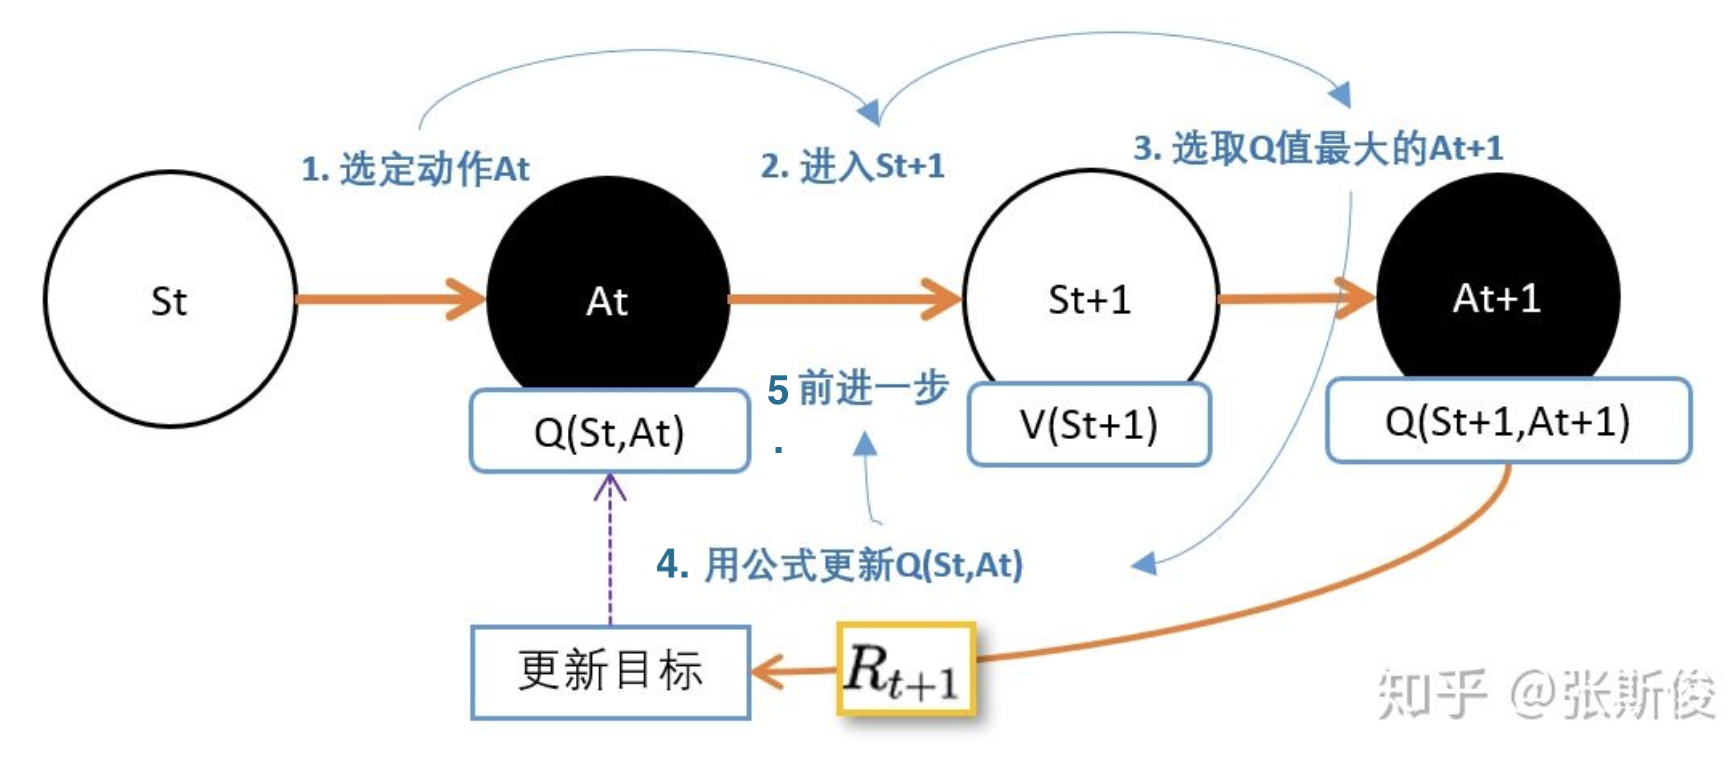
\includegraphics[width=.8\textwidth]{fig/ReinforcementLearning/RL_QLearning_EP.png}
\end{figure}

在具体实现的时候,有两个方式需要注意:Q-table 和 noisy-greedy。

\subsubsection{Q-table}
QLearning 算法非常适合用表格的方式进行存储和更新。所以一般我们会在开始时候,先创建一个 Q-tabel,也就是 Q 值表。这个表纵坐标是状态,横坐标是在这个状态下的动作。我们会初始化这个表的值为0。我们的任务就是,通过算法更新,把各个状态下的动作的Q值,填到上面去。
\begin{figure}[H]
    \centering
    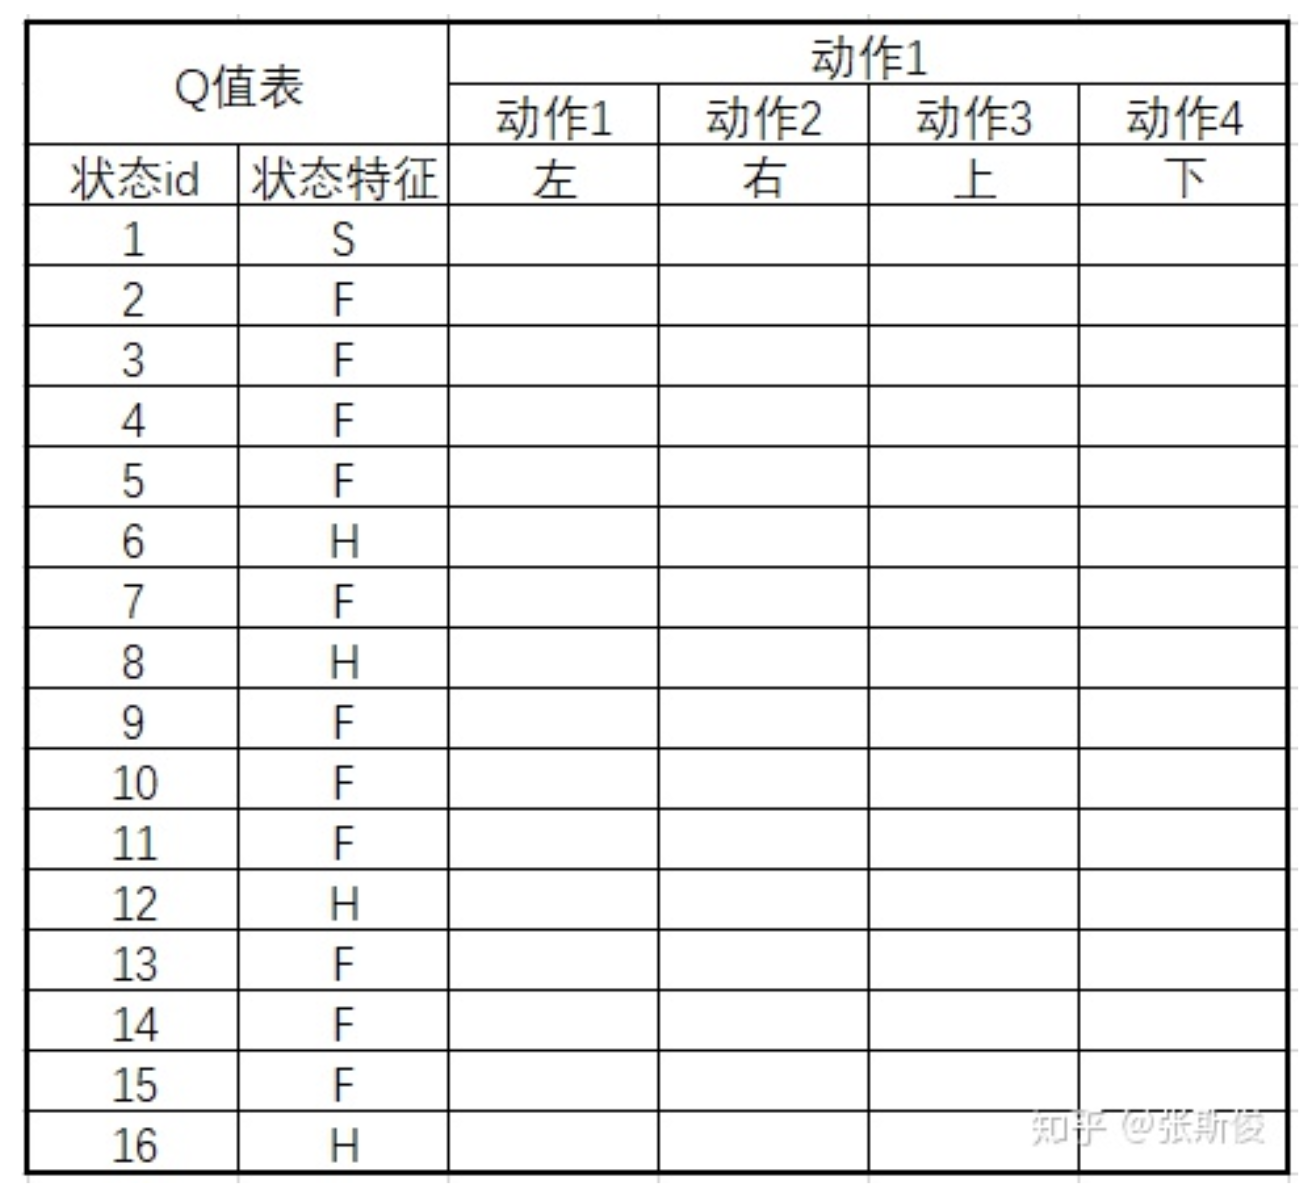
\includegraphics[width=.6\textwidth]{fig/ReinforcementLearning/RL_QLearning_QTable_Initial.png}
\end{figure}

\subsubsection{noisy-greedy}
我们解说过,在选择动作的时候,理论上每次都会使用当前状态下,Q 值最大的动作。这样的选择方式,我们称为“贪婪”(greedy)。

因为我们只选择Q值最大的动作,所以有一些动作没被更新过没有被选择的过的动作,将更新不到。Q值也永远为0。
\begin{figure}[H]
    \centering
    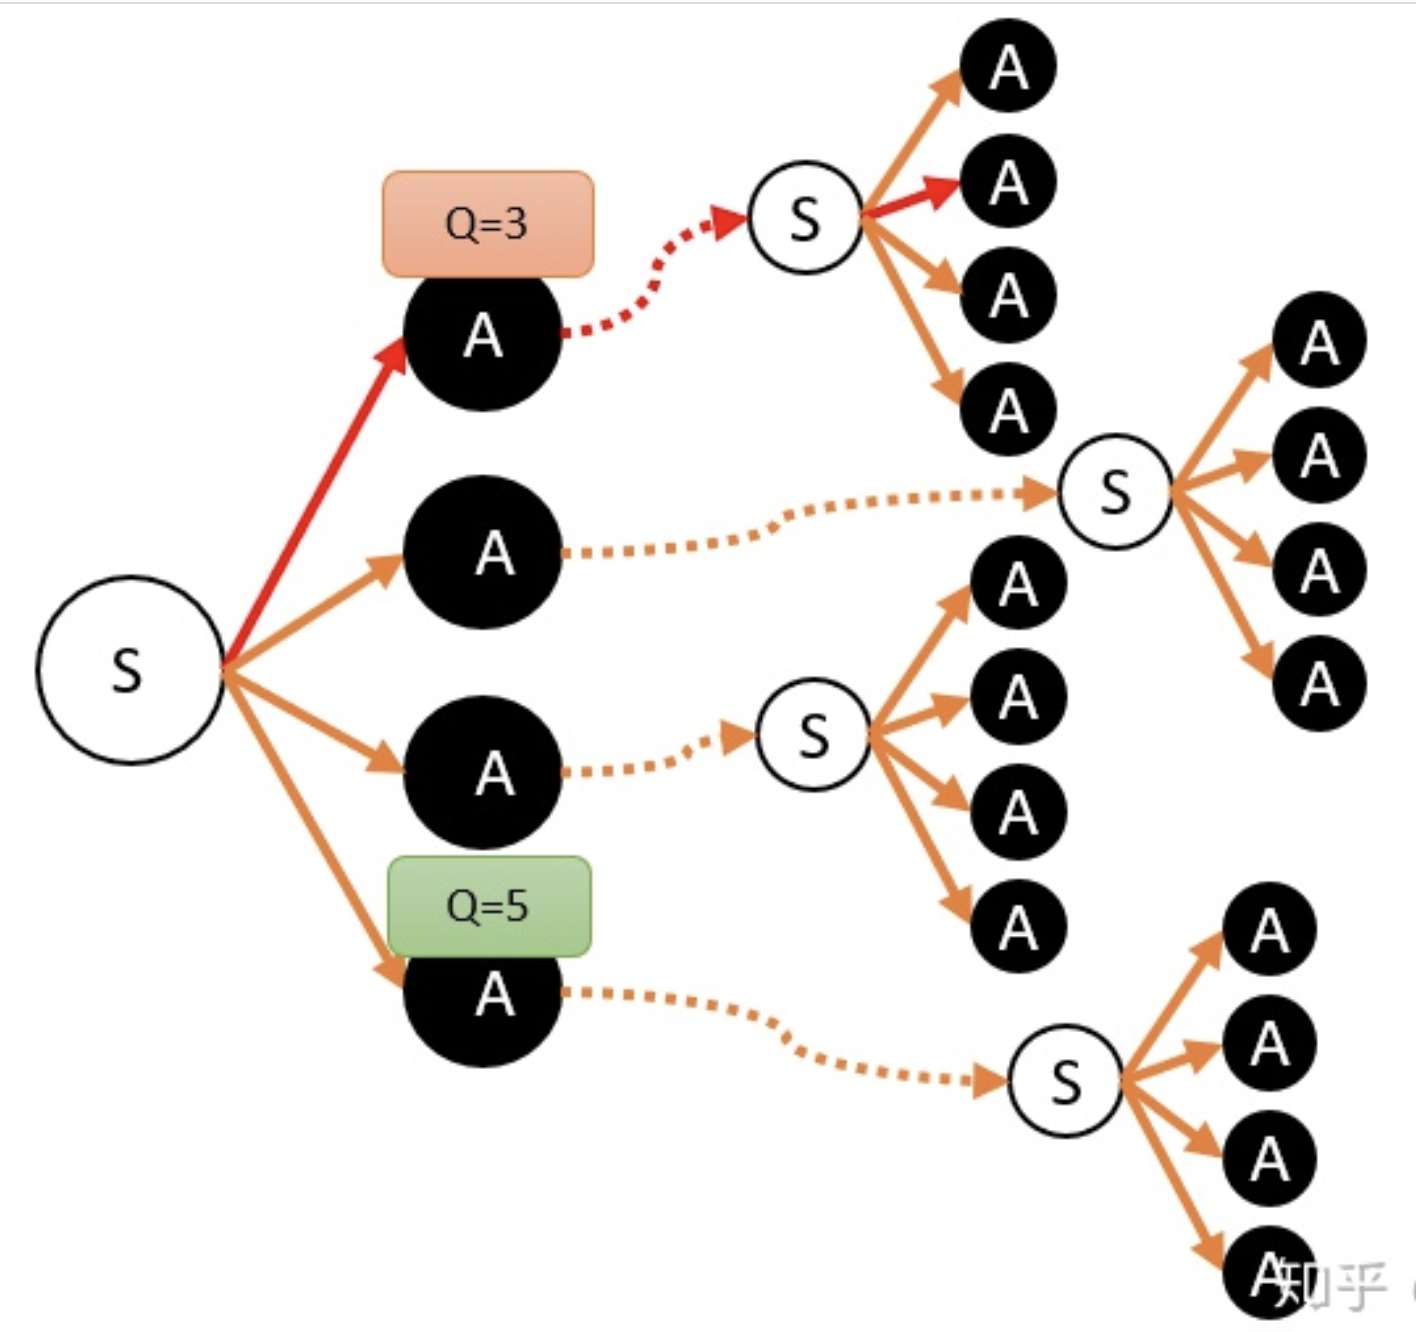
\includegraphics[width=.4\textwidth]{fig/ReinforcementLearning/RL_QLearning_Noisy_Greedy.png}
\end{figure}

假设某次智能体经过路径(途中的红色线路),根据 QLearning 算法更新公式,我们计算得到某动作 Q 值为3。由于其他动作还没执行过,因此他们保持初始值(一般为0)。按照贪婪算法,下一次智能体来到 S 的时候,会选择Q值最大的动作,也就是Q=3。于是红色路径再次被执行,Q值被更新。然后再一次,智能体仍然只会选红色线路。

但事实上,Q值最大的可能是其他的动作,但其他动作没有Q值,只是因为没有被“探索”出来。事实上我们会希望智能体在开始的时候更多随机行走去探索,而后面更多按照Q值去走动。

在每次选择动作的时候,就给我们要选择的动作叠加一个噪音。所谓噪音,就是在原来的值上增加一个随机值。
\begin{figure}[H]
    \centering
    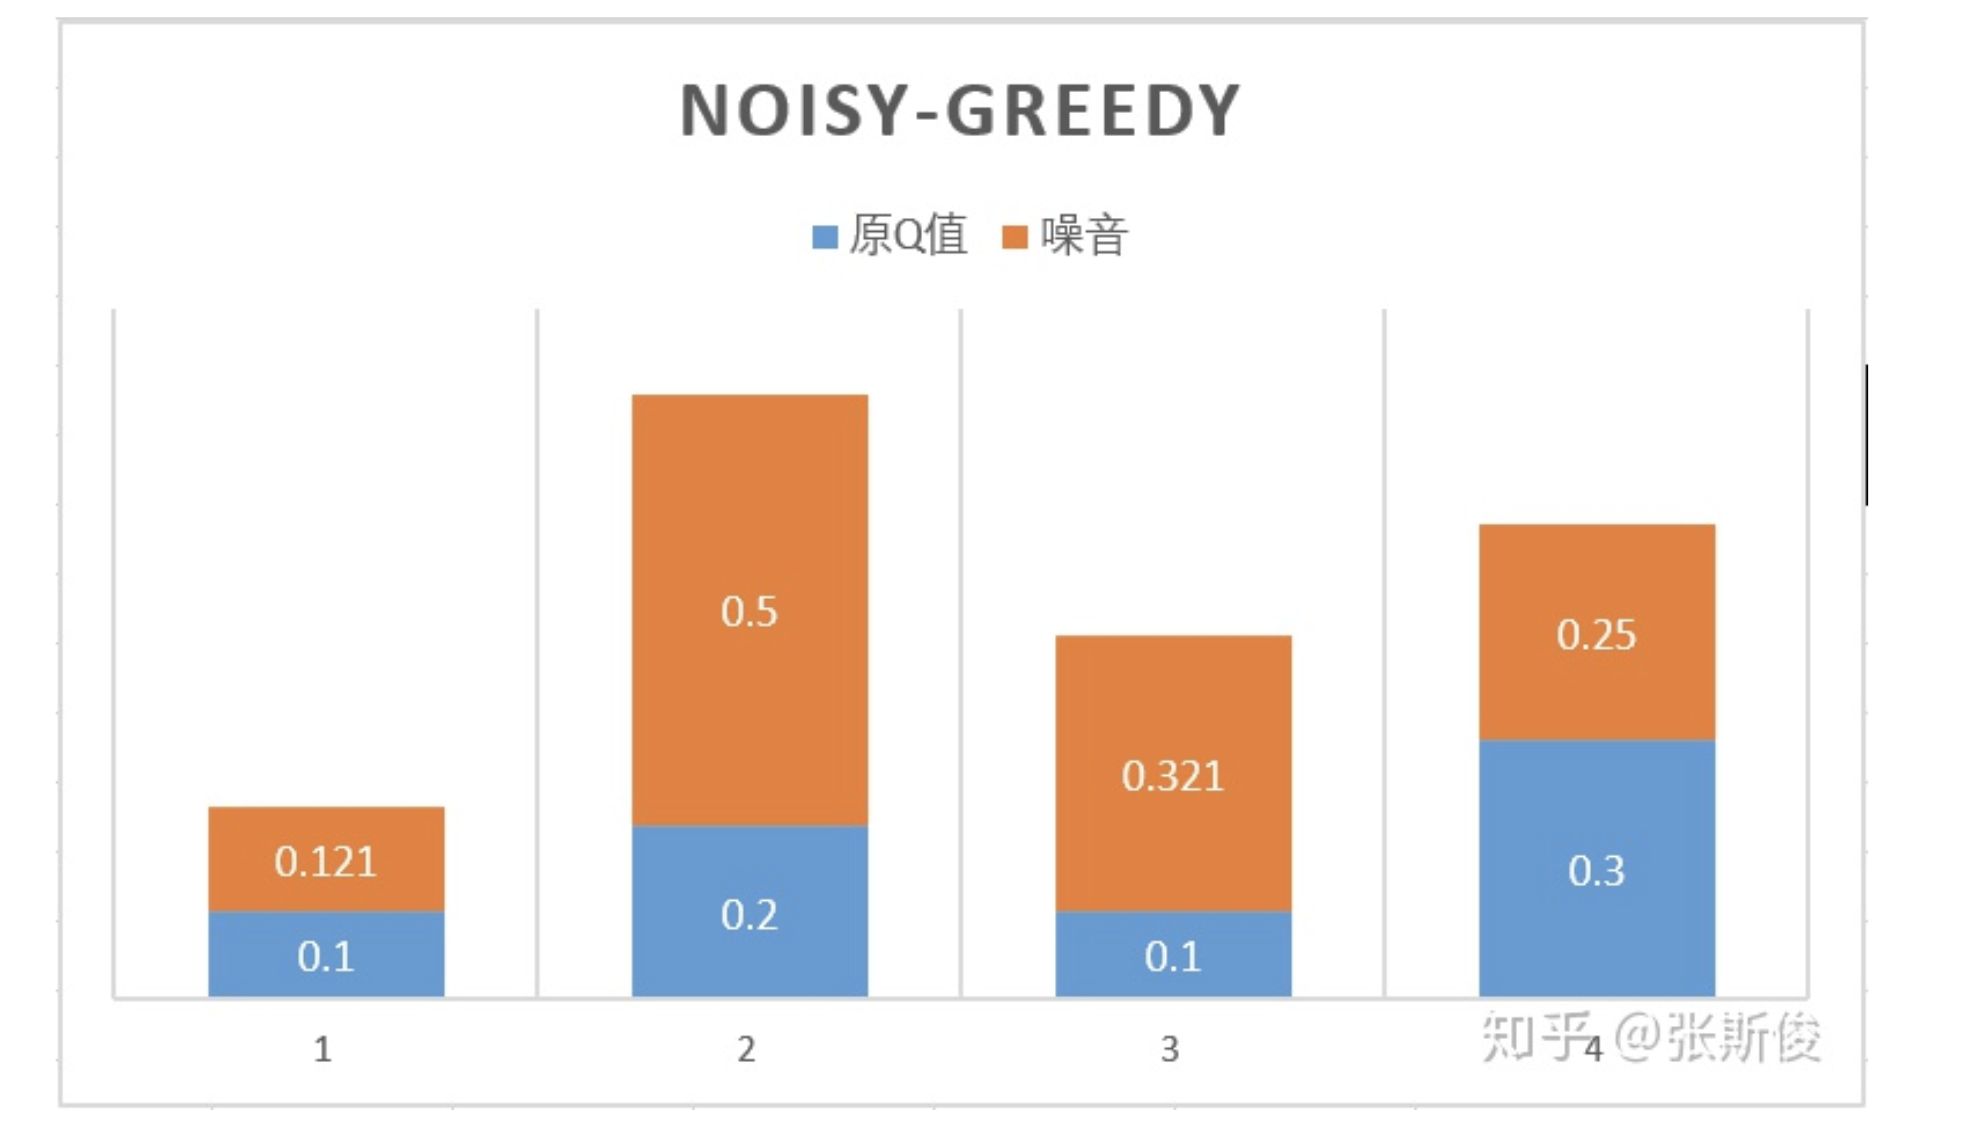
\includegraphics[width=.6\textwidth]{fig/ReinforcementLearning/RL_QLearning_Noisy_Greedy_Add_Noise.png}
\end{figure}
图中为某状态下,4个可选动作。 其中蓝色部分代表计算出来的Q值,也就是在Qtable上的值。 橙色部分是噪音,通过随机算法随机出来,每一次都会不同。可以看出来,原来蓝色部分 Q 值最大的是动作 4(0.3)。但在加上噪音之后,Q 值最大的是动作2(0.2+0.5)。所以最终智能体会选择动作 2。

所以,我们可以通过噪音来“干扰”智能体的选择,达到让智能体有更多探索的机会。注意!这些噪音只是在选择的时候,临时加上,每次都随机的。只干扰了当前选择,并不会影响真正的Q值。

当我们认为智能体对环境的了解已经足够充分,我们就可以慢慢减少噪音的大小。

在实做中,我们只需要在我们每次游戏后,将会减少产生噪音的方差,这样对干扰仍然有干扰,但这种干扰将会逐渐减少。直到相对于真正的 Q 值没有影响的程度。最终,agent 将会按照自己的策略选择动作。


\subsubsection{QLearning 总结}
Qlearning本质上是 TD(0) 算法,采用网格方式更新 Qtable。

Qlearning算法也有很大的局限性,我们看到,无论现实世界还是游戏世界,很多时候状态都是连续的,像表格这种方式,只能解决状态有限且离散的任务。于是就有了 DQN 算法用深度网络,解决了连续状态的问题。



\part{深度强化学习}
\section{DQN}
\subsection{DQN 介绍}
\subsubsection{DQN 和 QLearning 的关系}
DQN = Deep learning + Qleanrning。

Qleanrning有一个问题:只能解决格子类型离散型状态问题,对连续型状态束手无策。这是因为 Qlearning 在实做的时候用的是Q表格(Qtable)。但是神经网络,正好就能解决这个问题,因为神经网络是个函数。可以处理连续型的问题。


在Qlearning中,我们有一个Qtable,记录着在每一个状态下,各个动作的Q值。\textbf{Qtable的作用是当我们输入状态S,我们通过查表返回能够获得最大Q值的动作A。也就是我们需要找一个S-A的对应关系}。这个 S-A 的对应关系。可以用一个函数F表示:F(S) = A。这样我们就可以不用查表了,而且还有个好处,函数允许连续状态的表示。

这时候,深度神经网络就可以派上用场了。它的作用是:输入一个状态S,输出每个动作的Q值是多少。

\textcolor{red}{所以 Qlearning 和 DQN 并没有根本的区别。只是DQN用神经网络,也就是一个函数替代了原来Qtable而已。}

\subsubsection{神经网络的优化目标}
有监督学习的数据集中,有标签好的数据,就是神经网络要优化的目标。

在 Qlearning 中,我们用下一状态 $S_{t+1}$的最大Q值替代$S_{t+1}$的 V值。$V(S_{t+1})$加上状态转移产生的奖励R。就是Q(S,a) 的更新目标。也就是说用的是下一状态的Q值+奖励,作为更新的目标。如下图:
\begin{figure}[H]
    \centering
    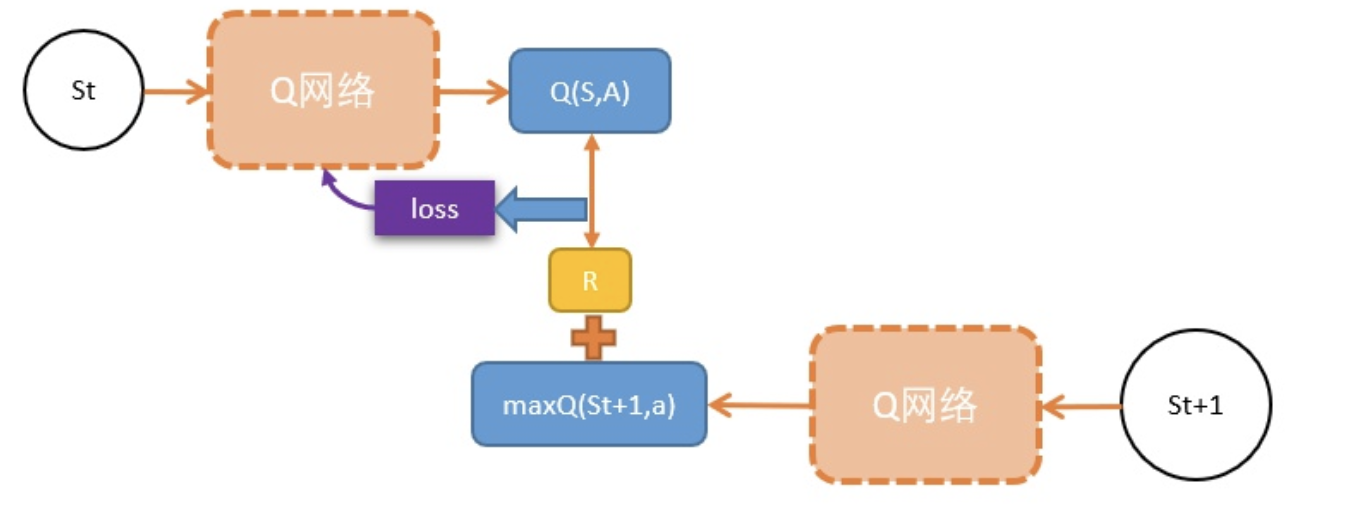
\includegraphics[width=1\textwidth]{fig/ReinforcementLearning/RL_DQN_Example.png}
\end{figure}

假设我们需要更新当前状态$S_t$下的某动作A的Q值:Q(S,A),我们可以这样做: 1. ; 2. ; 3.  4. 5. 

\begin{enumerate}
\setlength{\itemsep}{0pt}
\setlength{\parsep}{0pt}
\setlength{\parskip}{0pt}
    \item 执行A,往前一步,到达$S_{t+1}$;
    \item 把$S_{t+1}$输入Q网络,计算$S_{t+1}$下所有动作的Q值;
    \item 获得最大的Q值加上奖励R作为更新目标;
    \item 计算损失: Q(S,A)相当于有监督学习中的logits;$\max Q(S_{t+1}) + R$ 相当于有监督学习中的lables;用mse函数,得出两者的loss;
    \item 用loss更新Q网络。
\end{enumerate}

\textbf{也就是,我们用Q网络估算出来的两个相邻状态的Q值,他们之间的距离,就是一个r的距离。}

即 DQN 的更新公式如下(和 QLearning 的更新公式是一样的):
$$
Q(S,A) \leftarrow Q(S,A) + \alpha[R + \gamma Q(S', a) - Q(S,A)]
$$

\subsubsection{DQN总结}
(1)DQN就是Qlearning扔掉Qtable,换上深度神经网络。

(2)我们知道,解决连续型问题,如果表格不能表示,就用函数,而最好的函数就是深度神经网络。

(3)和有监督学习不同,深度强化学习中,我们需要自己找更新目标。通常在马尔科夫链体系下,两个相邻状态状态差一个奖励 r 经常能被利用。

\subsection{番外:强化学习的两个训练技巧}
\subsubsection{经验回放(Experience replay)}
在强化学习中,有一个问题始终绕不过。训练网络数据采集总是太慢。当然这个慢是对比网络训练的速度。在强化学习中,网络训练经过GPU的加速,比起游戏来时快很多的。所以训练的瓶颈一般在\textbf{智能体跟环境互动的过程中}。

如果我们能把互动过程中的数据,都存起来,当数据最够多的时候,再训练网络,那么就快很多了。经验回放(Experience replay)就是实现这样的过程:
\begin{itemize}
\setlength{\itemsep}{0pt}
\setlength{\parsep}{0pt}
\setlength{\parskip}{0pt}
    \item 我们把每一步的s,选择的a,进入新的状态s',获得的奖励r,新状态是否为终止状态,这些数据都全部存在一个叫回放缓存的地方(replay buffer);
    \item 当智能体与环境互动期间,就会不断产生这样一条一条数据。 数据1: 数据2: 数据3: ....;
    \item 当数据量足够,例如达到我们设定一个batch的大小,我们便从中抽出一个batch大小的数据,把这笔数据一起放入网络进行训练;
    \item 训练之后我们继续进行游戏,继续把新产生的数据添加到回放缓存里;
    \item 就这样,我们每次都随机抽出一个batch大小的数据训练智能体。这样,以前产生的数据同样也能用来训练数据了, 效率自然更高。
\end{itemize}

\subsubsection{固定Q目标(Fixed Q-targets)}
DQN的目标: $\gamma * \max Q(s') + r$
 
目标本身就包含一个Q网络,这样没有问题吗?理论上是没有问题的,但这样会造成Q网络的学习效率比较低,而且不稳定。如果把训练神经网络比喻成射击游戏,在target中有Q网络的话,就相当于在射击一个移动靶,因为每次射击一次,靶就会挪动一次。相比起固定的靶,无疑加上了训练的难度。

那怎么解决这个问题呢?既然现在是移动靶,那么我们就把它弄成是固定的靶,先停止10秒。10后挪动靶再打新的靶。这就是Fixed Q-targets的思路。
\begin{figure}[H]
    \centering
    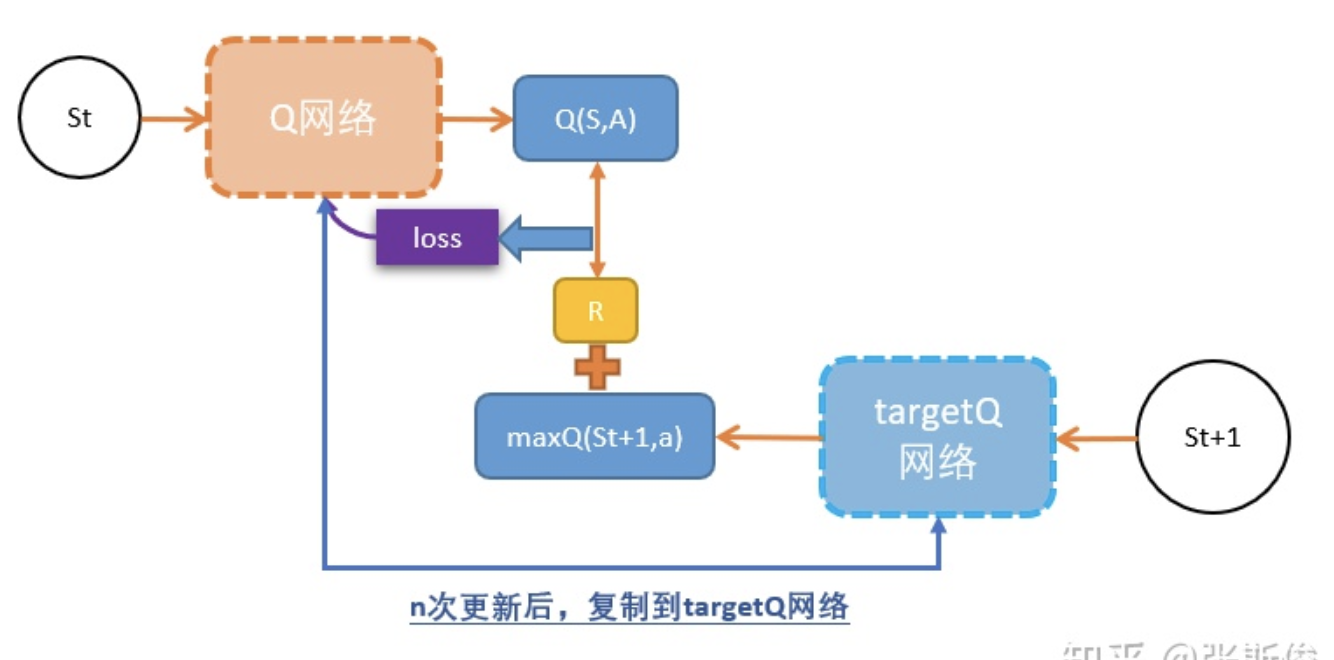
\includegraphics[width=.6\textwidth]{fig/ReinforcementLearning/RL_QLearning_Fix_Target.png}
\end{figure}

在实做的时候,其实和原来的DQN一样,唯一不同点是,我们用两个Q网络:

一个是原来的Q网络,用于估算Q(s);另外一个叫targetQ网络, targetQ自己并不会更新,也就是它在更新的过程中是固定的,用于计算更新目标。

$y = r + \gamma * \max(target Q(s'))$

我们进行N次更新后,就把新Q的参数赋值给旧Q。


\subsection{DQN的变种}
\subsubsection{Double DQN}
Double DQN 主要是为了解决一个问题:DQN对Q的估值通常会过大。直观地说,你可以这样认为: 我们用的是下一状态中,Q值最大的作为当前状态的估算。下一状态的Q值,以下下状态的最大Q值作为估算...这就有点像大话骰,这个Q值越传播就越大。那怎么办?用两个网络对Q进行预估,取最小的那个。就相当于,你们尽管吹牛,大的我不要,我要小的。当然,你会说这都可以?答案就是在试验当中,有奇效。这就是DoubleDQN的想法。

恰好,如果我们用上Fixed Q-targets,就是有两个Q网络了。

\subsubsection{Dueling DQN}
DuelingDQN也是一个比较容易实现的DQN变种,它和DQN的唯一差别,就是Network构造的不同。这种结构上的不同,可以让dueling DQN更快地学习到东西。

\section{策略梯度(PG)}
我们现在是把Q值和V值往死里算呀,但实际上,我们并不需要Q值呀,我们需要的是能获得最多的奖励总和呀。既然现在我们发明出宇宙最强无敌的Magic函数——神经网络。那我们直接用神经网络magic(s)=a不行吗?恭喜你,这就是PG的基本思想。PG用的是MC的G值来更新网络。也就是说,PG会让智能体一直走到最后。然后通过回溯计算G值。

于是得到S - A - G 的数据。这里的G就是对于状态S,选择了A的评分。也就是说: (1) 如果G值正数,那么表明选择A是正确的,我们希望神经网络输出A的概率增加。(鼓励) ; (2) 如果G是负数,那么证明这个选择不正确,我们希望神经网络输出A概率减少。(惩罚) ; (3) 而G值的大小,就相当于鼓励和惩罚的力度了。

我们分别以ABC三途路径作为例子:

\section{Actor-Critic}
我们知道,MC的效率是相对比较低的,因为需要一直走到最终状态。所以我们希望用TD代替MC。那么我们可不可以把PG和DQN结合呢?

注意:这里是一个大坑。个人更倾向于把AC理解成PG的TD版本,而不是PG+DQN。

这是为什么呢?Critic网络负责估算Q值 Actor网络负责估算策略。这不是很完美吗?但我们要注意,Q值都是正数,容易掉进“正数陷阱”。假设我们用Critic网络,预估到S状态下三个动作A1,A2,A3的Q值分别为1,2,10。但在开始的时候,我们采用平均策略,于是随机到A1。于是我们用策略梯度的带权重方法更新策略,这里的权重就是Q值。于是策略会更倾向于选择A1,意味着更大概率选择A1。结果A1的概率就持续升高...

那要怎么办?我们把Q值弄成有正有负就可以了。一堆数减去他们的平均值一定有正有负吧!Q减去Q的期望值,也就是V值,就可以得到有正有负的Q了。

也就是说Actor用Q(s,a)-V(s)去更新。但我们之前也说过Q和V都要估算太麻烦了。能不能只统一成V呢?

\section{PPO}
略

\section{DDPG}
略


\section{TD3}


\section{A3C和DPPO}






















%\printbibliography
\bibliography{../ref}
\bibliographystyle{IEEEtran}
\end{document}